\chapter{Dynamical Systems}
\label{chap:dynsys}

Near the end of Chapter \ref{chap:eigen}, we have talked about systems of first-order linear ODEs which are actually the prototype of \textit{linear} dynamical systems. A \textit{dynamical system} describes the change or evolution (\textit{dynamics}) of multiple variables (\textit{state}) in time that can depend on the variables themselves as well as the time coordinate. Starting from a particular initial point (\textit{particle}) in the physical/state space, a deterministic trajectory will be traced by the particle as the dynamical system operates. We will derive several important ideas like equilibrium points and their types, starting from the easier linear dynamical systems, and then generalize to the more complicated \textit{non-linear} dynamical systems where the gap can often be bridged by the \textit{Hartman-Grobman Theorem} if the linearized equilibrium point in question is a \textit{hyperbolic equilibrium point}. Finally, we will discuss the prime example of non-linear dynamical systems in Earth Science, the \textit{Lorenz-63 Model} which demonstrates the phenomenon of \textit{chaos}.

\section{Linear Dynamical Systems}

\subsection{Types of Equilibrium Points in Two-dimensional Linear Dynamical Systems}

We will motivate the notions of equilibrium points and their types from the perspective of the relatively simpler two-dimensional linear dynamical systems. Recalling Definition \ref{defn:1ordODEsys}, such dynamical systems may be succinctly described by
\begin{align}
\left\{\begin{alignedat}{1}
\dfrac{dx}{dt} &= \alpha_1^{(1)} x + \alpha_2^{(1)} y \\
\dfrac{dy}{dt} &= \alpha_1^{(2)} x + \alpha_2^{(2)} y   
\end{alignedat}\right.
\label{eqn:2ddynexplicit}
\end{align}
where $\alpha_j^{(i)}$ are constant coefficients and there are no time-dependent forcing terms. Alternatively, in matrix form, it is
\begin{align}
\textbf{y}' = A\textbf{y} \label{eqn:17.2}
\end{align}
where $\textbf{y} = (x,y)^T$ and
\begin{align}
A = 
\begin{bmatrix}
\alpha_1^{(1)} & \alpha_2^{(1)} \\
\alpha_1^{(2)} & \alpha_2^{(2)} 
\end{bmatrix}
\label{eqn:2ddynexplicit2}
\end{align}
An \index{Equilibrium Point}\keywordhl{equilibrium point} of a dynamical system is where the R.H.S. vanishes (i.e.\ $\textbf{y}' = \textbf{0}$) so that the time derivatives are zeros and the variables (or physically, a \index{Particle}\textit{particle}) become stationary. The characteristics of the trajectories/\index{Orbit}\textit{orbits} near these equilibrium points are important and can be readily inferred from their types.
\begin{defn}[Equilibrium Points of a Dynamical System]
\label{defn:eqpts}
An equilibrium point $\tilde{\textbf{y}}$ of a \textit{time-independent} dynamical system
\begin{align}
\frac{d\textbf{y}}{dt} = F(\textbf{y}) \label{eqn:eqpts1}
\end{align}
where $F$ is a vector of functions that only depend on the state $\textbf{y}$, satisfies
\begin{align}
F(\tilde{\textbf{y}}) = \textbf{0} \label{eqn:eqpts2}
\end{align}
\end{defn}
It is not hard to see that the origin $\textbf{0}$ is automatically an (only) equilibrium point for the linear dynamical system in (\ref{eqn:17.2}) if $A$ is invertible\footnote{If $A$ is not invertible, it means that there exists a non-trivial null space for $A$ (Properties \ref{proper:invertrank}) and by Definition \ref{defn:nullspace} this null space $\mathcal{N}(A)$ will be a subspace (straight line) where for $\tilde{\textbf{y}} \in \mathcal{N}(A)$, $\tilde{\textbf{y}}' = A\tilde{\textbf{y}} = \textbf{0}$ so there will be an "equilibrium line" instead and it becomes a degenerate case.} and we will focus on this scenario. As we have seen in Section \ref{section:sysode}, the characteristics (growth/decay/spiral centered at the origin) are largely determined by the eigenvalues of $A$ through diagonalization, assumed possible. Specifically, by Properties \ref{proper:diagODE} the solution trajectories/orbits (\index{Field Lines}\keywordhl{field lines}) for (\ref{eqn:17.2}) will be described by $z_1 = c_1e^{\lambda_1 t}$, $z_2 = c_2e^{\lambda_2 t}$ where $\lambda_1, \lambda_2$ are the respective eigenvalues of $A$ and $\textbf{z} = (z_1, z_2)^T$ denotes the transformed coordinates in the basis formed by the eigenvectors $\textbf{v}_1$, $\textbf{v}_2$. The family of trajectories in the original physical state space will then be in the form of
\begin{align}
\textbf{y} = c_1\textbf{v}_1e^{\lambda_1 t} + c_2\textbf{v}_2e^{\lambda_2 t} \label{eqn:eigendyn2d}
\end{align}
According to this, we can determine the types of equilibrium points at the origin based on the eigenvalues $\lambda_1, \lambda_2$ of the coefficient matrix $A$ for any two-dimensional linear dynamical system.
\begin{proper}[Types of Equilibrium Points for Two-dimensional Linear Dynamical Systems]
\label{proper:2dequiltypes}
Given a two-dimensional dynamical system $\textbf{y}' = A\textbf{y}$ where $A$ is a real $2 \times 2$ matrix, denote the eigenvalues of $A$ by $\lambda_1$ and $\lambda_2$ which are exactly the roots of the characteristic polynomial of $A$. Further assume that $A$ is invertible such that there is no eigenvalue of pure zero, i.e.\ $\lambda_j \neq 0$ (Theorem \ref{thm:singularzeroeig}). The equilibrium point at the origin $\tilde{\textbf{y}} = \textbf{0}$ can be classified into different types depending on the following three situations.
\begin{enumerate}
    \item If the characteristic polynomial has two distinct real roots, then it is
    \begin{enumerate}[label=(\alph*)]
        \item a \index{Source}\index{Unstable Node}\keywordhl{source (unstable node)} where the field lines emanate from it if both of the eigenvalues are positive, i.e.\ $\lambda_1, \lambda_2 > 0$;
        \item a \index{Sink}\index{Stable Node}\keywordhl{sink (stable node)} where the field lines converge to it if both of the eigenvalues are negative, i.e.\ $\lambda_1, \lambda_2 < 0$; 
        \item otherwise, a \index{Saddle Point}\keywordhl{saddle point} where the field lines are deflected away from it if one of the eigenvalues is positive and the other one is negative. i.e.\ $\lambda_1 > 0, \lambda_2 < 0$.
    \end{enumerate}
    \item Else if, the characteristic polynomial has a repeated real root $\lambda_1 = \lambda_2 = \lambda_p$, then it is
    \begin{enumerate}[label=(\alph*)]
        \item a source if $\lambda_p > 0$;
        \item a sink if $\lambda_p < 0$; 
    \end{enumerate}
    where for simplicity we require that the geometric multiplicity of the repeated eigenvalue is equal to its algebraic multiplicity $= 2$, and thus $A$ is diagonalizable.
    \item Otherwise, the characteristic polynomial has two complex conjugate roots $\lambda_1 = a+bi$, $\lambda_2 = a-bi$, $b \neq 0$, then
    \begin{enumerate}[label=(\alph*)]
        \item an \index{Unstable Spiral}\keywordhl{outward/unstable spiral (source)} if $a > 0$;
        \item an \index{Stable Spiral}\keywordhl{inward/stable spiral (sink)} if $a < 0$;
        \item a \index{Center}\keywordhl{center} if $a = 0$;
    \end{enumerate}
\end{enumerate}
\end{proper}
These various types of equilibrium points in a two-dimensional space are summarized in Table \ref{tab:equilpts} below. Again, assume that the matrix $A$ can be diagonalized into 
\begin{align*}
D = 
\begin{bmatrix}
\lambda_1 & 0 \\
0 & \lambda_2
\end{bmatrix}
\end{align*}
as suggested by Properties \ref{proper:diagonalize}, then due to Properties \ref{proper:similarinvariant}, the trace $\tr(A) = \lambda_1 + \lambda_2$ and determinant $\det(A) = \lambda_1\lambda_2$ will remain invariant. These are exactly the sum and product of the roots for the characteristic polynomial and by high school algebra we can readily infer the signs of the two eigenvalues from them. Moreover, we can know if the roots belong to the case of real and distinct, real and repeated, or complex conjugates, by calculating the discriminant $\Delta = \tr(A)^2 - 4\det(A)$ from the characteristic polynomial 
\begin{align*}
p(\lambda) &= (\lambda_1 - \lambda)(\lambda_2 - \lambda) \\
&= \lambda_1\lambda_2 - (\lambda_1 + \lambda_2)\lambda + \lambda^2 \\
&= \det(A) - \tr(A)\lambda + \lambda^2
\end{align*}
which is also invariant. Hence we can determine the different types of equilibrium points (Situations 1 and 3 in Properties \ref{proper:2dequiltypes})\footnote{Situation 2 is a bit special since our assumption may be violated where the geometric multiplicity of the repeated eigenvalue is now only $1$, i.e.\ deficient, and it becomes degenerate.} solely from the trace and determinant of $A$ (see the three rightmost columns in Table \ref{tab:equilpts}). The classification and the corresponding phase portraits are visualized in Figure \ref{fig:phasediagram} as follows.
\begin{table}[ht!]
    \centering
    \small
    \begin{tabular}{|p{40pt}|p{48pt}|p{68pt}|p{44pt}|c|c|c|}
    \hline
    Type of Roots & Signs of Roots & Type of Equilibrium Points & Stability & $\tr(A)$ & $\det(A)$ & $\Delta$ \\
    \hline
    \multirow{3}{40pt}{Two Distinct Real Roots} & Both Positive & Source (Unstable Node) & Unstable & $(+)$ & $(+)$ & $(+)$ \\
    \hhline{~------}
     & Both Negative & Sink (Stable Node) & Stable & $(-)$ & $(+)$ & $(+)$ \\
    \hhline{~------} 
    & One Positive, One Negative & Saddle Point & Unstable & Any & $(-)$ & $(+)$ \\
    \hline
    \multirow{2}{40pt}{One Repeated (Real) Root} & Positive & Source (Unstable Node) & Unstable & $(+)$ & $(+)$ & $0$ \\
    \hhline{~------}
     & Negative & Sink (Stable Node) & Stable & $(-)$ & $(+)$ & $0$ \\
    \hline
    \multirow{3}{40pt}{Two Complex (Conjugate) Roots} & Positive Real Part & Outward / Unstable Spiral & Unstable & $(+)$ & $(+)$ & $(-)$ \\
    \hhline{~------}
     & Negative Real Part & Inward / Stable Spiral & Stable & $(-)$ & $(+)$ & $(-)$ \\
    \hhline{~------} 
    & Zero Real Part & Center & Stable & $0$ & $(+)$ & $(-)$ \\
    \hline
    \end{tabular}
    \caption{\textit{Types and attributes of equilibrium points in a two-dimensional dynamical system. The discriminant is $\Delta = \tr(A)^2 - 4\det(A)$.}}
    \label{tab:equilpts}
\end{table}

\tikzset{decorated arrows/.style={
    postaction={
        decorate,
        decoration={
            markings,
            mark={at position 0.5 with {\arrow{stealth}}},}
}}}

\begin{figure}
    \centering
    \begin{tikzpicture}
    \draw[thick, ->] (-6,0) -- (6,0) node[right]{$\tr(A)$};
    \draw[thick, ->] (0,-6) -- (0,6) node[above]{$\det(A)$};
    \node[below left]{$O$}; 
    \draw[gray, thick] plot[domain=-4.5:4.5,samples=100] (\x, {(\x)^2/4});
    \node[gray, rotate=-58] at (-3.6,2.5) {$\Delta = \tr(A)^2 - 4\det(A) = 0$};
    \node[gray, rotate=58] at (3.1,3) {Complex};
    \node[gray, rotate=58] at (3.6,2.5) {Real};
    \node[anchor=center, Green, rotate=90] at (-6, 5) {\large Stable};
    \node[anchor=center, Red, rotate=-90] at (6, 5) {\large Unstable};
    \coordinate (saddle) at (0,-3);
    \node[anchor=center, blue] at (0, -5) {Saddle Point};
    \begin{axis}[at=(saddle), anchor=center, scale=0.5, xmin=-2, xmax=2, ymin=-2, ymax=2,
    axis lines=center, hide axis]
    \addplot[domain=-1:1.5,samples=50,blue,decorated arrows] ({0.5*e^(x) + 0.5*e^(-x)},{0.5*e^(x) - 1*e^(-x)});
    \addplot[domain=-1.5:2,samples=50,blue,decorated arrows] ({0.3*e^(x) + 0.3*e^(-x)},{0.3*e^(x) - 0.6*e^(-x)});
    \addplot[domain=-1:1.5,samples=50,blue,decorated arrows] ({0.5*e^(x) - 0.5*e^(-x)},{0.5*e^(x) + 1*e^(-x)});
    \addplot[domain=-1.5:2,samples=50,blue,decorated arrows] ({0.3*e^(x) - 0.3*e^(-x)},{0.3*e^(x) + 0.6*e^(-x)});
    \addplot[domain=-1:1.5,samples=50,blue,decorated arrows] ({-(0.5*e^(x) + 0.5*e^(-x))},{-(0.5*e^(x) - 1*e^(-x))});
    \addplot[domain=-1.5:2,samples=50,blue,decorated arrows] ({-(0.3*e^(x) + 0.3*e^(-x))},{-(0.3*e^(x) - 0.6*e^(-x))});
    \addplot[domain=-1:1.5,samples=50,blue,decorated arrows] ({-(0.5*e^(x) - 0.5*e^(-x))},{-(0.5*e^(x) + 1*e^(-x))});
    \addplot[domain=-1.5:2,samples=50,blue,decorated arrows] ({-(0.3*e^(x) - 0.3*e^(-x))},{-(0.3*e^(x) + 0.6*e^(-x))});
    \addplot[domain=0:2,samples=50,blue,decorated arrows] ({-x},{-x});
    \addplot[domain=0:2,samples=50,blue,decorated arrows] ({x},{x});
    \addplot[domain=0:2,samples=50,blue,decorated arrows] ({-0.5*(2-x)},{(2-x)});
    \addplot[domain=0:2,samples=50,blue,decorated arrows] ({0.5*(2-x)},{-(2-x)});
    \end{axis}
    \node[anchor=center, blue] at (0, 1) {Center};
    \coordinate (center) at (0,3);
    \begin{axis}[at=(center), anchor=center, scale=0.5, xmin=-2, xmax=2, ymin=-2, ymax=2,
    axis lines=center, hide axis]
    \addplot[domain=0:360,samples=50,blue,decorated arrows] ({1*(cos(x)) + 0.8*(sin(x))},{-1*(cos(x)) + 1*(sin(x))});
    \addplot[domain=0:360,samples=50,blue,decorated arrows] ({2/3*(cos(x)) + 1.6/3*(sin(x))},{-2/3*(cos(x)) + 2/3*(sin(x))});
    \addplot[domain=0:360,samples=50,blue,decorated arrows] ({1/3*(cos(x)) + 0.8/3*(sin(x))},{-1/3*(cos(x)) + 1/3*(sin(x))});
    \end{axis}
    \node[anchor=center, blue] at (-3, 8) {Stable Spiral};
    \coordinate (stablespir) at (-3, 6);
    \begin{axis}[at=(stablespir), anchor=center, scale=0.5, xmin=-2, xmax=2, ymin=-2, ymax=2,
    axis lines=center, hide axis]
    \addplot[domain=0:1.99,samples=200,blue,decorated arrows] ({1*(2-x)*(sin(2*deg(ln(2-x))) - 0.5*(2-x)*(cos(2*deg(ln(2-x)))},{1*(2-x)*(cos(2*deg(ln(2-x))) + 0.5*(2-x)*(sin(2*deg(ln(2-x)))});
    \addplot[domain=0:1.99,samples=200,blue,decorated arrows] ({-1*(2-x)*(sin(2*deg(ln(2-x))) + 0.5*(2-x)*(cos(2*deg(ln(2-x)))},{-1*(2-x)*(cos(2*deg(ln(2-x))) - 0.5*(2-x)*(sin(2*deg(ln(2-x)))});
    \addplot[domain=0:1.99,samples=200,blue,decorated arrows] ({1*(2-x)*(sin(2*deg(ln(2-x))) + 0.5*(2-x)*(cos(2*deg(ln(2-x)))},{1*(2-x)*(cos(2*deg(ln(2-x))) - 0.5*(2-x)*(sin(2*deg(ln(2-x)))});
    \addplot[domain=0:1.99,samples=200,blue,decorated arrows] ({-1*(2-x)*(sin(2*deg(ln(2-x))) - 0.5*(2-x)*(cos(2*deg(ln(2-x)))},{-1*(2-x)*(cos(2*deg(ln(2-x))) + 0.5*(2-x)*(sin(2*deg(ln(2-x)))});
    \end{axis}
    \node[anchor=center, blue] at (3, 8) {Unstable Spiral};
    \coordinate (unstablespir) at (3, 6);
    \begin{axis}[at=(unstablespir), anchor=center, scale=0.5, xmin=-2, xmax=2, ymin=-2, ymax=2,
    axis lines=center, hide axis]
    \addplot[domain=0.01:2,samples=200,blue,decorated arrows] ({1*x*(cos(2*deg(ln(x)))},{0.8*(x)*(sin(2*deg(ln(x)))});
    \addplot[domain=0.01:2,samples=200,blue,decorated arrows] ({-1*x*(cos(2*deg(ln(x)))},{-0.8*(x)*(sin(2*deg(ln(x)))});
    \end{axis}
    \node[anchor=center, blue] at (-5.5, 3) {Sink};
    \coordinate (sink) at (-5, 1);
    \begin{axis}[at=(sink), anchor=center, scale=0.5, xmin=-2, xmax=2, ymin=-2, ymax=2,
    axis lines=center, hide axis]
    \addplot[domain=0:1.5,samples=200,blue,decorated arrows] ({0.6*(1.5-x) + 0.6*(1.5-x)^2},{-0.6*(1.5-x) + 0.6*(1.5-x)^2});
    \addplot[domain=0:1.5,samples=200,blue,decorated arrows] ({1*(1.5-x) + 0.2*(1.5-x)^2},{-1*(1.5-x) + 0.2*(1.5-x)^2});
    \addplot[domain=0:1.5,samples=200,blue,decorated arrows] ({-0.6*(1.5-x) + 0.6*(1.5-x)^2},{0.6*(1.5-x) + 0.6*(1.5-x)^2});
    \addplot[domain=0:1.5,samples=200,blue,decorated arrows] ({-1*(1.5-x) + 0.2*(1.5-x)^2},{1*(1.5-x) + 0.2*(1.5-x)^2});
    \addplot[domain=0:1.5,samples=200,blue,decorated arrows] ({-(0.6*(1.5-x) + 0.6*(1.5-x)^2)},{-(-0.6*(1.5-x) + 0.6*(1.5-x)^2)});
    \addplot[domain=0:1.5,samples=200,blue,decorated arrows] ({-(1*(1.5-x) + 0.2*(1.5-x)^2)},{-(-1*(1.5-x) + 0.2*(1.5-x)^2)});
    \addplot[domain=0:1.5,samples=200,blue,decorated arrows] ({-(-0.6*(1.5-x) + 0.6*(1.5-x)^2)},{-(0.6*(1.5-x) + 0.6*(1.5-x)^2)});
    \addplot[domain=0:1.5,samples=200,blue,decorated arrows] ({-(-1*(1.5-x) + 0.2*(1.5-x)^2)},{-(1*(1.5-x) + 0.2*(1.5-x)^2)});
    \addplot[domain=0:1.5,samples=100,blue,decorated arrows]({1*(1.5-x)},{-1*(1.5-x)});
    \addplot[domain=0:1.5,samples=100,blue,decorated arrows]({-1*(1.5-x)},{1*(1.5-x)});
    \addplot[domain=0:1.5,samples=100,blue,decorated arrows]({0.6*(1.5-x)^2},{0.6*(1.5-x)^2});
    \addplot[domain=0:1.5,samples=100,blue,decorated arrows]({-0.6*(1.5-x)^2},{-0.6*(1.5-x)^2});
    \end{axis}
    \node[anchor=center, blue] at (5.5, 3) {Source};
    \coordinate (source) at (5, 1);
    \begin{axis}[at=(source), anchor=center, scale=0.5, xmin=-2, xmax=2, ymin=-2, ymax=2,
    axis lines=center, hide axis]
    \addplot[domain=0:1.5,samples=200,blue,decorated arrows] ({0.8*x^1.5 + 0.2*x},{-0.4*x^1.5 + 0.6*x});
    \addplot[domain=0:1.5,samples=200,blue,decorated arrows] ({-0.8*x^1.5 + 0.2*x},{0.4*x^1.5 + 0.6*x});
    \addplot[domain=0:1.5,samples=200,blue,decorated arrows] ({-(0.8*x^1.5 + 0.2*x)},{-(-0.4*x^1.5 + 0.6*x)});
    \addplot[domain=0:1.5,samples=200,blue,decorated arrows] ({-(-0.8*x^1.5 + 0.2*x)},{-(0.4*x^1.5 + 0.6*x)});
    \addplot[domain=0:1.5,samples=200,blue,decorated arrows] ({-1.2*x^1.5},{0.6*x^1.5});
    \addplot[domain=0:1.5,samples=200,blue,decorated arrows] ({1.2*x^1.5},{-0.6*x^1.5});
    \addplot[domain=0:1.5,samples=200,blue,decorated arrows] ({0.3*x},{0.9*x});
    \addplot[domain=0:1.5,samples=200,blue,decorated arrows] ({-0.3*x},{-0.9*x});
    \end{axis}
    \end{tikzpicture}
    \caption{\textit{Different types of equilibrium points and their representative phase portraits categorized according to the trace and determinant of the coefficient matrices for the family of two-dimensional dynamical systems.}}
    \label{fig:phasediagram}
\end{figure}

\begin{exmp}
\label{exmp:2d3dyn}
Identify the type of equilibrium point at the origin for the three two-dimensional dynamical systems $\textbf{y}' = A\textbf{y}$ where the coefficient matrices $A = $ 
\begin{enumerate}[label=(\alph*)]
    \item $\left[\begin{array}{@{\,}wc{10pt}wc{10pt}wc{10pt}@{}}
    -1 & 4 \\
    2 & 1
    \end{array}\right]$
    \item $\left[\begin{array}{@{\,}wc{10pt}wc{10pt}wc{10pt}@{}}
    3 & 2 \\
    1 & 3
    \end{array}\right]$
    \item $\left[\begin{array}{@{\,}wc{10pt}wc{10pt}wc{10pt}@{}}
    -1 & -1 \\
    2 & -1
    \end{array}\right]$
\end{enumerate}
\end{exmp}
\begin{solution}
We simply do the classification according to Table \ref{tab:equilpts}. For case (a), the trace is $\tr(A) = (-1) + 1 = 0$, the determinant is $\det(A) = (-1)(1) - (4)(2) = -9 < 0$ and the discriminant is $\Delta = (0)^2 - 4(-9) = 36 > 0$, so it corresponds to a saddle point. Similarly, for case (b), we have $\tr(A) = 3 + 3 = 6 > 0$, $\det(A) = (3)(3) - (2)(1) = 7 > 0$ and $\Delta = (6)^2 - 4(7) = 8 > 0$, thus it is an unstable node. Finally, for case (c), $\tr(A) = (-1) + (-1) = -2 < 0$, $\det(A) = (-1)(-1) - (2)(-1) = 3 > 0$ and $\Delta = (-2)^2 - 4(3) = -8 < 0$ and therefore it is a stable spiral. The stream plots of these three dynamical systems are shown in Figure \ref{fig:2d3dyn}. 
\end{solution}

\begin{figure}[ht!]
    \centering
    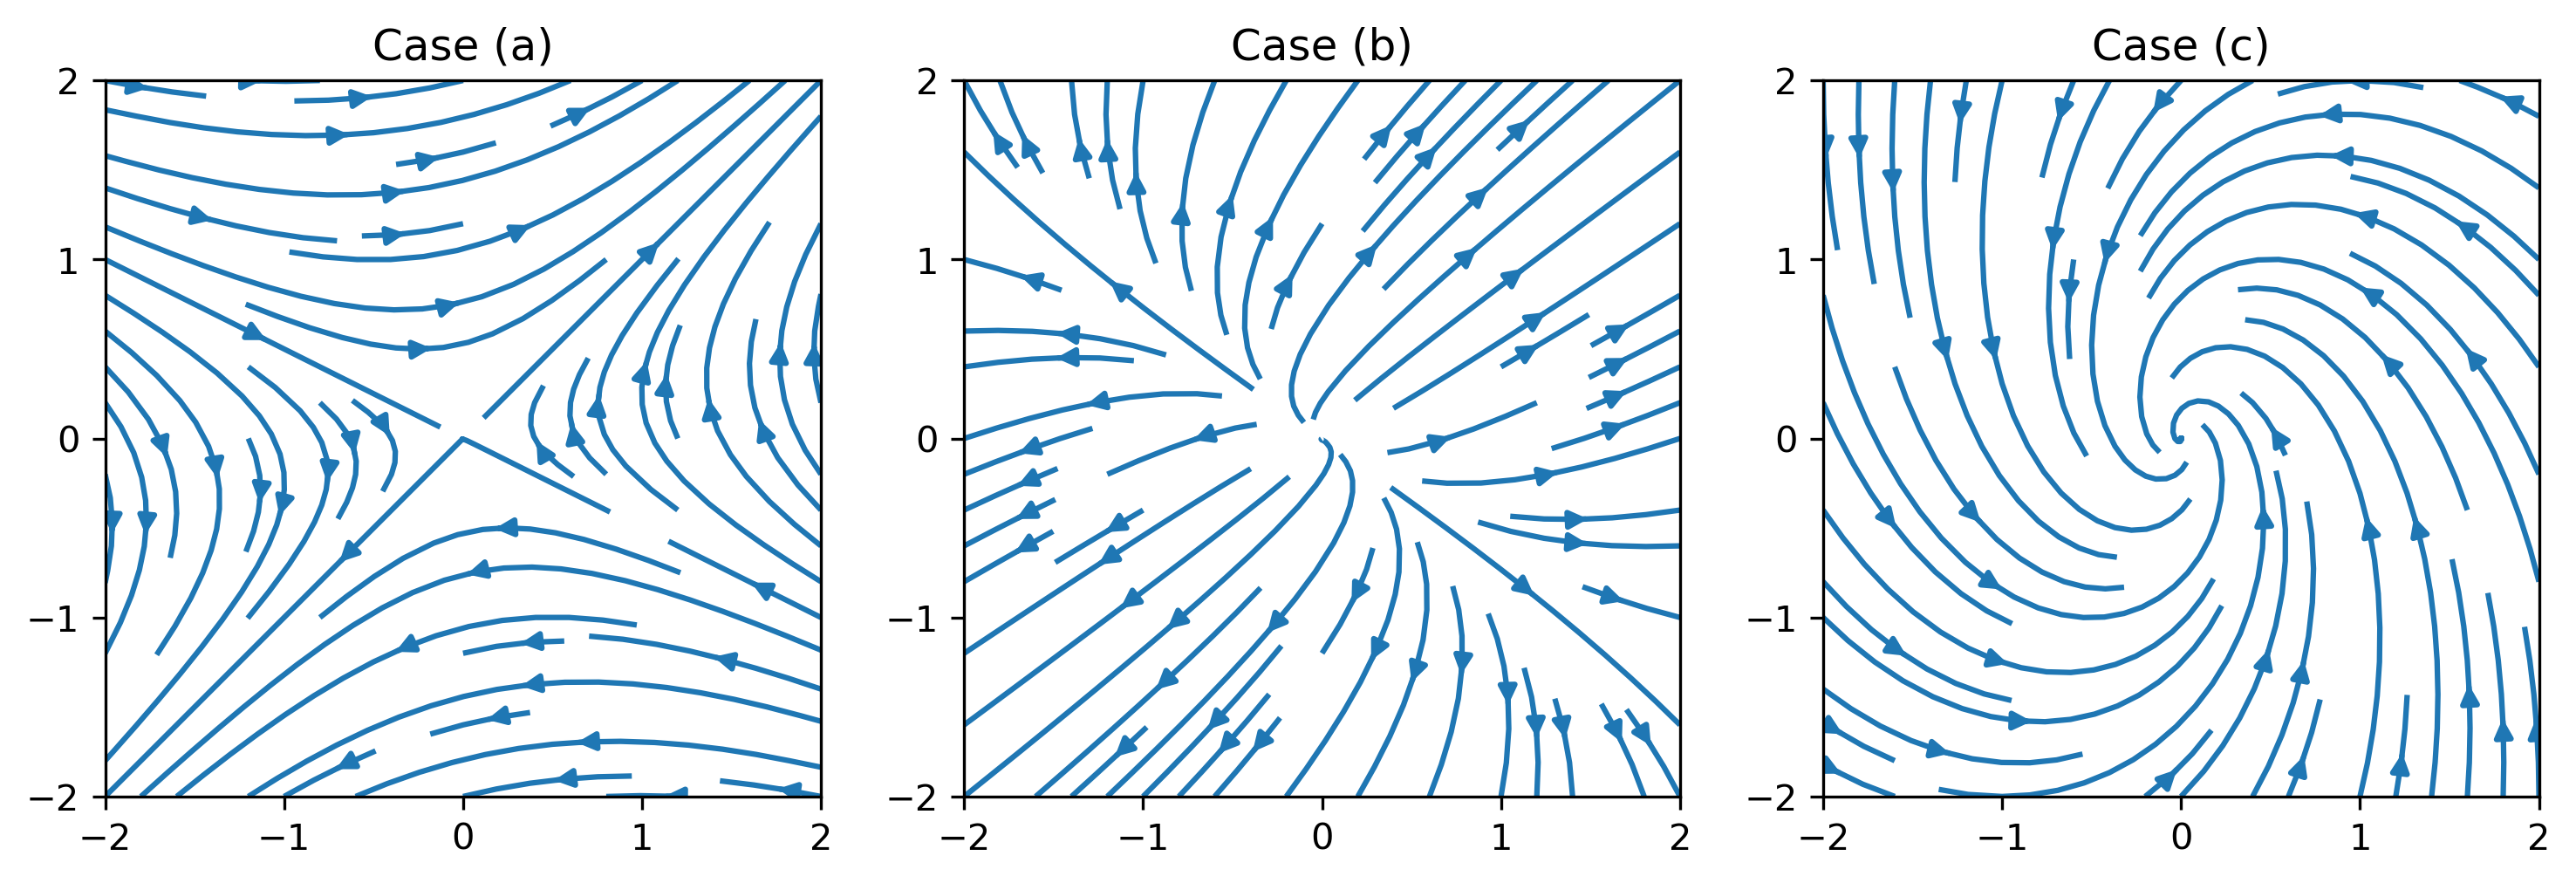
\includegraphics[width=\textwidth]{graphics/3exmps2ddynamic.png}
    \caption{\textit{The stream plots for the three two-dimensional dynamical systems in Example \ref{exmp:2d3dyn}.}}
    \label{fig:2d3dyn}
\end{figure}

\subsection{Generalization to Time-independent Forcings and Higher-dimensional Linear Dynamical Systems}

Sometimes there will be an additional forcing term on the R.H.S. of the linear dynamical system that represents external processes. Let's further assume that it is time-independent just like the dynamical system itself before, so that we have
\begin{align}
\frac{d\textbf{y}}{dt} = A\textbf{y} + \textbf{G}
\end{align}
where $\textbf{G}$ is a constant vector with the same dimension as the state vector $\textbf{y}(t)$. As in Properties \ref{proper:2dequiltypes}, we require that $A$ is invertible, and hence by Theorem \ref{thm:sqlinsysunique} there exists a unique solution $\tilde{\textbf{y}}$ for the linear system $A\textbf{y} = -\textbf{G}$. Subsequently, the dynamical system can be rewritten into
\begin{align}
\frac{d\textbf{y}(t)}{dt} = A\textbf{y}(t) - A\tilde{\textbf{y}} = A(\textbf{y}(t) - \tilde{\textbf{y}})     
\end{align}
where a linear change of variable $\delta\textbf{y}(t) = \textbf{y}(t) - \tilde{\textbf{y}}$ will make it become
\begin{align}
\frac{d(\delta\textbf{y}(t))}{dt} = A(\delta\textbf{y}(t)) 
\label{eqn:translateddynsys}
\end{align}
which is essentially the same as (\ref{eqn:17.2}) but with $\delta\textbf{y}(t)$ in place of $\textbf{y}(t)$. Therefore, both the qualitative and quantitative behaviors of the dynamical system will also be the same, except that the equilibrium point is now located by $\delta \textbf{y} = 0$, i.e.\ moved to $\textbf{y} = \tilde{\textbf{y}}$ instead of the original $\textbf{y} = \textbf{0}$. This effectively translates the equilibrium point and the entire corresponding phase portrait by a displacement of $\tilde{\textbf{y}}$, and the results from the previous discussion can thus be readily applied to linear dynamical systems with a time-independent forcing. Particularly, for a two-dimensional linear dynamical system as in (\ref{eqn:2ddynexplicit}), if we add an additional time-independent term so that it now looks like
\begin{align}
\left\{\begin{alignedat}{1}
\dfrac{dx}{dt} &= \alpha_1^{(1)} x + \alpha_2^{(1)} y + G_x \\
\dfrac{dy}{dt} &= \alpha_1^{(2)} x + \alpha_2^{(2)} y + G_y 
\end{alignedat}\right.
\end{align}
where $(G_x, G_y)^T = \textbf{G}$ are some fixed constants, and $\tilde{\textbf{y}} = (\tilde{x}, \tilde{y})^T$ is the unique solution to the linear system $A\textbf{y} = -\textbf{G}$ with $A$ in the form of (\ref{eqn:2ddynexplicit2}) and invertible such that
\begin{align}
\left\{\begin{alignedat}{1}
\alpha_1^{(1)} \tilde{x} + \alpha_2^{(1)} \tilde{y} &= -G_x \\
\alpha_1^{(2)} \tilde{x} + \alpha_2^{(2)} \tilde{y} &= -G_y 
\end{alignedat}\right.
\end{align}
then the dynamical system can be recast as
\begin{align}
&\left\{\begin{alignedat}{1}
\dfrac{dx}{dt} - \dfrac{d\tilde{x}}{dt} &= \alpha_1^{(1)} x + \alpha_2^{(1)} y - \alpha_1^{(1)} \tilde{x} + \alpha_2^{(1)} \tilde{y} \\
\dfrac{dy}{dt} - \dfrac{d\tilde{y}}{dt} &= \alpha_1^{(2)} x + \alpha_2^{(2)} y - \alpha_1^{(2)} \tilde{x} + \alpha_2^{(2)} \tilde{y} 
\end{alignedat}\right. \nonumber \\
&\left\{\begin{alignedat}{1}
\dfrac{d(x-\tilde{x})}{dt} &= \alpha_1^{(1)} (x-\tilde{x}) + \alpha_2^{(1)} (y-\tilde{y}) \\
\dfrac{d(y-\tilde{y})}{dt} &= \alpha_1^{(2)} (x-\tilde{x}) + \alpha_2^{(2)} (y-\tilde{y})
\end{alignedat}\right. \nonumber \\
\Rightarrow &\left\{\begin{alignedat}{1}
\dfrac{d(\delta x)}{dt} &= \alpha_1^{(1)} \delta x + \alpha_2^{(1)} \delta y \\
\dfrac{d(\delta y)}{dt} &= \alpha_1^{(2)} \delta x + \alpha_2^{(2)} \delta y
\end{alignedat}\right.
\label{eqn:2ddynfull}
\end{align}
which is essentially the same as (\ref{eqn:2ddynexplicit}) but with displacements from the newly translated equilibrium point $\delta x$ and $\delta y$ replacing the $x$ and $y$ coordinates that are initially relative to the origin.
\begin{exmp}
Locate the equilibrium point for the two-dimensional linear dynamical system
\begin{align*}
\left\{\begin{alignedat}{1}
\dfrac{dx}{dt} &= -5x + 2y + 8 \\
\dfrac{dy}{dt} &= x - 4y + 2
\end{alignedat}\right.
\end{align*}
and determined its type.
\end{exmp}
\begin{solution}
First, the position of the equilibrium point is found by solving the linear system
$A\textbf{y} = -\textbf{G}$ where
\begin{align*}
A &= 
\begin{bmatrix}
-5 & 2 \\
1 & -4
\end{bmatrix}
&
\textbf{G} &= 
\begin{bmatrix}
G_x \\
G_y
\end{bmatrix}
=
\begin{bmatrix}
8 \\
2
\end{bmatrix}
\end{align*}
It can be checked that the solution is
\begin{align*}
\tilde{\textbf{y}} = \begin{bmatrix}
2 \\
1
\end{bmatrix}
\end{align*}
as
\begin{align*}
\begin{bmatrix}
-5 & 2 \\
1 & -4
\end{bmatrix}
\begin{bmatrix}
2 \\
1
\end{bmatrix}
=
\begin{bmatrix}
-8 \\
-2
\end{bmatrix}
=
-\begin{bmatrix}
8 \\
2
\end{bmatrix}
\end{align*}
and thus the equilibrium point is at $\tilde{\textbf{y}} = (2,1)^T$. Next, translate the coordinate system so that it is now relative to this equilibrium point by writing $\delta x = x - 2$ and $\delta y = y - 1$. The dynamical system now looks like
\begin{align*}
&\left\{\begin{alignedat}{1}
\dfrac{d(x-2)}{dt} &= -5(x-2) + 2(y-1) \\
\dfrac{d(y-1)}{dt} &= (x-2) - 4(y-1)
\end{alignedat}\right. \\
&\left\{\begin{alignedat}{1}
\dfrac{d(\delta x)}{dt} &= -5\delta x + 2\delta y \\
\dfrac{d(\delta y)}{dt} &= \delta x - 4\delta y
\end{alignedat}\right.
\end{align*}
the one in (\ref{eqn:translateddynsys}) and the type of this equilibrium point can then be inferred from Table \ref{tab:equilpts}. The trace, determinant and discriminant are $\tr(A) = (-5) + (-4) = -9 < 0$, $\det(A) = (-5)(-4) - (1)(2) = 18 > 0$ and $\Delta = (-9)^2 - 4(18) = 9 > 0$, and therefore it is a stable node located at $(2,1)^T$.
\end{solution}

Another generalization to be made is for higher-dimensional dynamical systems. The logic in (\ref{eqn:eigendyn2d}) and Properties \ref{proper:2dequiltypes} remains the same. For a dynamical system $\textbf{y}' = A\textbf{y}$ of any dimension, let's say $n$, denote all the pair of eigenvalues and eigenvectors by $\lambda_j$ and $\smash{\vec{v}_\lambda^{(j)}}$, $j = 1, 2, \ldots, n$. Then the subspace spanned by those $\smash{\vec{v}_\lambda^{(j)}}$ with negative real $\lambda_j$ form the stable part of a node, and in contrast, those with positive real $\lambda_j$ form the unstable part of a node. If there are both stable and unstable parts, then they will give rise to an overall saddle point. The subspace spanned by a pair of $\smash{\vec{v}_\lambda^{(j)}}$ with the eigenvalues $\lambda_j$ being complex conjugates will lead to an unstable spiral if their real part is positive, a stable spiral if their real part is negative, and a center if it is exactly zero. The characteristic of the equilibrium point can be viewed either separately or together in these different subspaces (more formally known as \textit{"manifolds"} in this context).

\section{Non-linear Dynamical Systems}

\subsection{Heuristic Understandings of Stability and Attractiveness}
% https://math.stackexchange.com/questions/4453028/why-an-lti-system-with-some-zero-eigenvalues-still-stable
Before moving from linear dynamical systems to non-linear dynamical systems, we will take a detour to visit the concepts of stability and attractiveness. Heuristically, stability means that if the particle starts close enough to the equilibrium point, then it will always remain close to the equilibrium point. Meanwhile, attractiveness means that if it starts close enough to the equilibrium point likewise, then it will eventually be absorbed to that equilibrium point. We give the formal definitions for both of them below.
\begin{defn}
For a time-independent dynamical system as given by (\ref{eqn:eqpts1}) in Definition \ref{defn:eqpts}, an equilibrium point $\tilde{\textbf{y}}$ that satisfies (\ref{eqn:eqpts2}) is
\begin{enumerate}[label=(\alph*)]
    \item \index{Stable}\keywordhl{stable}, if for all $\epsilon > 0$, there exists an $\eta(\epsilon) > 0$\footnotemark{} such that $\norm{\textbf{y}(\textbf{y}_0, 0) - \tilde{\textbf{y}}} \leq \eta$ implies that $\norm{\textbf{y}(\textbf{y}_0, t) - \tilde{\textbf{y}}} \leq \epsilon$ for all $t \geq 0$;
    \item \index{Attractive}\keywordhl{attractive}, if there exists an $\eta > 0$ such that $\norm{\textbf{y}(\textbf{y}_0, 0) - \tilde{\textbf{y}}} \leq \eta$ implies that $\norm{\textbf{y}(\textbf{y}_0, t) - \tilde{\textbf{y}}} \to 0$ as $t \to \infty$.
\end{enumerate}
where $\textbf{y}(\textbf{y}_0, t)$ denotes the position of the particle at time $t$ with an initial condition (starting point) of $\textbf{y}_0 = \textbf{y}(\textbf{y}_0, 0)$. An equilibrium point is \index{Asymptotically Stable}\keywordhl{asymptotically stable} if it is both stable and attractive, and simply \index{Unstable}\keywordhl{unstable} if it is not stable.
\end{defn}
\footnotetext{Note that $\eta(\epsilon) \leq \epsilon$ implicitly. The definitions here and the following discussion are largely based on this \href{https://math.stackexchange.com/questions/4453028/why-an-lti-system-with-some-zero-eigenvalues-still-stable}{Math Stackexchange post} (4453028).} Translated to plain language, it means that the equilibrium point is stable if, for all particles starting inside a ball centered at the equilibrium point with a small radius of $\eta$, their subsequent trajectories will be contained within another ball with a small radius of $\epsilon$ at all times, whereas it is attractive if all particles starting inside some ball with a small radius of $\eta$ will converge to the equilibrium point as the time goes to infinity. It may be tempting to say that an attractive equilibrium point will be automatically (asymptotically) stable but there are some subtle differences between these two, demonstrated in the following counter-example. Consider the non-linear two-dimensional dynamical system
\begin{align}
&\left\{\begin{alignedat}{1}
\dfrac{dx}{dt} &= x^2 - y^2 \\
\dfrac{dy}{dt} &= 2xy
\end{alignedat}\right. 
\label{eqn:magneticdipolefield}
\end{align}
The pattern of its field lines is shown in Figure \ref{fig:magneticdipolefield}. 
\begin{figure}
    \centering
    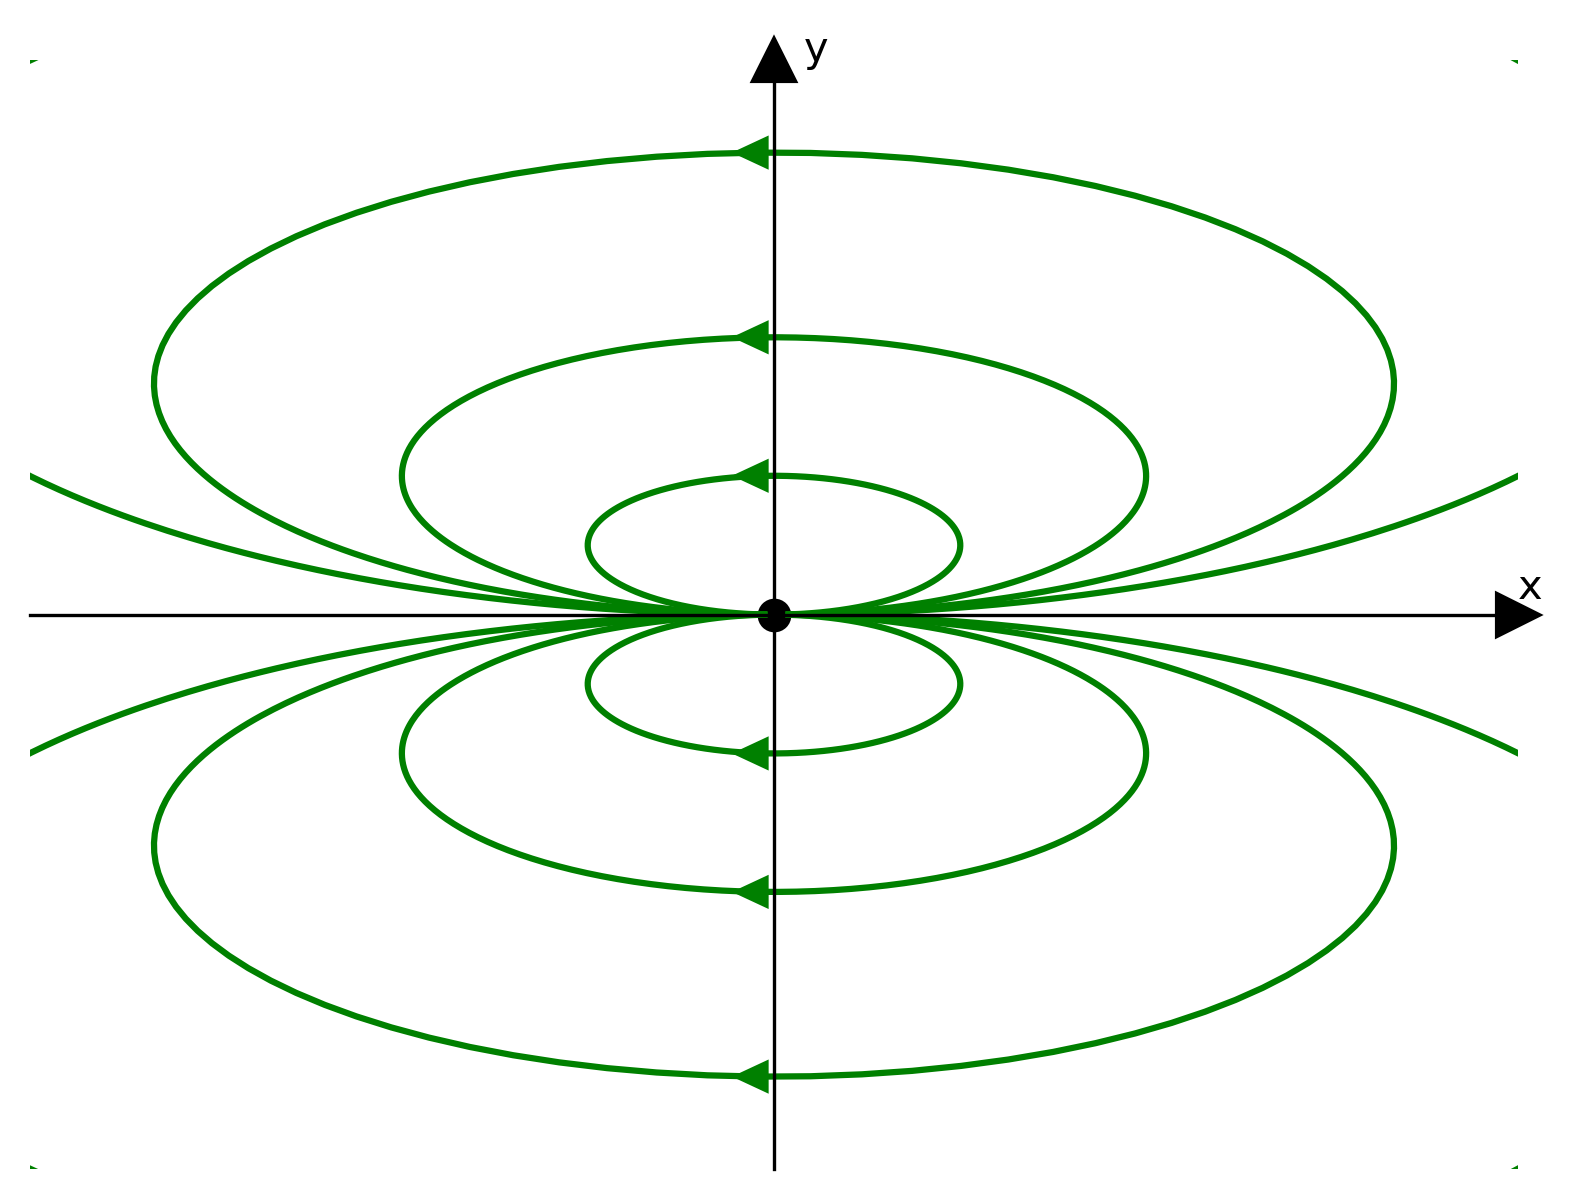
\includegraphics[scale=0.6]{graphics/dipolefield.png}
    \caption{\textit{Field lines for the non-linear dynamical system (\ref{eqn:magneticdipolefield}).}}
    \label{fig:magneticdipolefield}
\end{figure}
The field lines are akin to the \textit{magnetic dipole} type. The equilibrium point at the origin is attractive as all outgoing field lines will return to the equilibrium point, but is also unstable since we can always find a more outer field line that travels farther in both the $x$ and $y$-directions.\footnotemark{} Nevertheless, all stable equilibrium types in Table \ref{tab:equilpts} except centers, are attractive and hence asymptotically stable.

\subsection{Linearization and Hartman-Grobman Theorem}
\label{subsection:HGthm}

Since non-linear dynamical systems are more complex, we may want to reduce them to the more familiar, linear dynamical systems. Motivated by the form (\ref{eqn:translateddynsys}), we seek to approximate the behavior of orbits near a non-linear equilibrium point by
\begin{align}
\frac{d(\delta y_i(t))}{dt} = \sum_{j=1}^{n} A_{ij}(\delta y_j (t)) = \sum_{j=1}^{n} \alpha_{j}^{(i)}(\delta y_j(t)) \label{eqn:dynapproxproto}
\end{align}
where $\delta y_i$ represents a small displacement from the equilibrium point in the $i$-th direction, and each of the R.H.S. is a linear function of the displacement components with constant coefficients \smash{$\alpha_{j}^{(i)}$}. Then, the previous (\ref{eqn:2ddynfull}) shows the fully written-out form of this approximation applicable to a two-dimensional dynamical system. Using Taylor Expansion to the first order from Multivariable Calculus, the non-linear dynamical system that takes the general form of (\ref{eqn:eqpts1}), or written in component form\footnotetext{There is a caveat to this "counter-example" though. The "central" field line (not explicitly drawn out) that starts from $y = 0$ to the right of the equilibrium point will keep accelerating along the $x$-axis and diverges so it is only \textit{almost} attractive. In fact, it is impossible to have an unstable, yet \textit{truly} attractive equilibrium point if the dynamical system is smooth enough. However, the key takeaway is to help the readers distinguish between the concepts of stability and attractiveness, and this example should be adequate.} 
\begin{align}
\frac{d y_i}{dt} = F_i(\textbf{y})
\end{align}
can be readily approximated by
\begin{align}
\frac{d(y_i(t) - \tilde{y}_i)}{dt} \approx F_i(\tilde{\textbf{y}}) + \sum_{j=1}^{n} \left(\left.\frac{\partial F_i}{\partial y_j}\right|_{\tilde{\textbf{y}}}\right) (y_j(t) - \tilde{y}_j) + O({\delta y_j}^2)
\end{align}
near the equilibrium point $\tilde{\textbf{y}}$ where \smash{$\partial F_i/\partial y_j|_{\tilde{\textbf{y}}}$} is the partial derivative of $F_i$ along the $j$-th direction evaluated at the equilibrium point. The matrix formed by \smash{$\partial F_i/\partial y_j$} is known as the \index{Jacobian (Matrix)}\keywordhl{Jacobian (matrix)}. Due to Definition \ref{defn:eqpts} of equilibrium points (\ref{eqn:eqpts2}), $F_i(\tilde{\textbf{y}}) = 0$, and if we further discard the higher-order error terms $O({\delta y_j}^2)$ it becomes
\begin{align}
\frac{d(\delta y_i(t))}{dt} = \sum_{j=1}^{n}  \left(\left.\frac{\partial F_i}{\partial y_j}\right|_{\tilde{\textbf{y}}}\right) \delta y_j(t) \label{eqn:nonlindynjac}
\end{align}
Comparing with the proposed form in (\ref{eqn:dynapproxproto}), we immediately identity the required coefficients \smash{$\alpha_{j}^{(i)}$} with \smash{$\partial F_i/\partial y_j|_{\tilde{\textbf{y}}}$}. For a two-dimensional non-linear dynamical system, the corresponding fully written-out form is then
\begin{align}
&\left\{\begin{alignedat}{1}
\dfrac{d(\delta x)}{dt} &= \dfrac{\partial F_1}{\partial x}(\tilde{x}, \tilde{y}) \delta x + \dfrac{\partial F_1}{\partial y}(\tilde{x}, \tilde{y}) \delta y \\
\dfrac{d(\delta y)}{dt} &= \dfrac{\partial F_2}{\partial x}(\tilde{x}, \tilde{y}) \delta x + \dfrac{\partial F_2}{\partial y}(\tilde{x}, \tilde{y}) \delta y
\end{alignedat}\right.
\end{align}
Now, the problem is whether such a \index{Linearization}\keywordhl{linearization} of the non-linear equilibrium point can successfully capture its characteristics. To proceed, we first introduce a class of equilibrium points known as \index{Hyperbolic Equilibrium Point}\keywordhl{hyperbolic equilibrium points}.
\begin{defn}[Hyperbolic Equilibrium Points]
For a linear dynamical system as formulated by (\ref{eqn:translateddynsys}), 
a hyperbolic equilibrium point is an equilibrium point where all the eigenvalues of $A$ have non-zero real parts. Similarly, for a non-linear dynamical system, a hyperbolic equilibrium point is an equilibrium point where all the eigenvalues of the Jacobian matrix $A_{ij} = \smash{\partial F_i/\partial y_j|_{\tilde{\textbf{y}}}}$ in the linearization by (\ref{eqn:nonlindynjac}) have non-zero real parts, evaluated at the equilibrium point.
\end{defn}
By this criteria, in Table \ref{tab:equilpts}, the stable/unstable nodes, saddle points, and stable/unstable spirals are all hyperbolic equilibrium points. The only exception is the centers, in addition to other omitted degenerate cases where at least one of the eigenvalues is strictly zero. Since stable equilibrium types excluding centers are all asymptotically stable as noted at the end of the last subsection, hyperbolic equilibrium points are either asymptotically stable or unstable. Now we are ready to examine the major result about hyperbolic equilibrium points, the \index{Linearization Theorem}\index{Hartman-Grobman Theorem}\keywordhl{Hartman-Grobman (Linearization) Theorem}, which states that the qualitative behavior of orbits near a non-linear hyperbolic equilibrium point will be the same as its linearization.
\begin{thm}[Hartman-Grobman Theorem]
\label{thm:HGthm}
A hyperbolic equilibrium point $\tilde{\textbf{y}}$ of any non-linear dynamical system that has a Jacobian of $\smash{\partial F_i/\partial y_j|_{\tilde{\textbf{y}}}}$, belongs to the same type and has the same qualitative behavior in its neighborhood as the corresponding linear hyperbolic equilibrium point, with the matrix $A$ in (\ref{eqn:translateddynsys}) equal to this Jacobian $\smash{\partial F_i/\partial y_j|_{\tilde{\textbf{y}}}}$.
\end{thm}
Unfortunately, for an equilibrium point that is not hyperbolic, we need other methods to determine its behavior which are out of the scope of this book. Anyway, let's see how the Hartman-Grobman Theorem can be applied in the following example.
\begin{exmp}
\label{exmp:nonlindynsaddlenode}
Find all the equilibrium points for the two-dimensional non-linear dynamical system
\begin{align*}
\left\{
\begin{aligned}
\frac{dx}{dt} &= y - xy \\
\frac{dy}{dt} &= x - xy
\end{aligned}
\right.
\end{align*}
\end{exmp}
\begin{solution}
Since the dynamical system is now non-linear we can have multiple isolated equilibrium points. A simple rewriting of the dynamical system shows that
\begin{align*}
\left\{
\begin{aligned}
\frac{dx}{dt} &= y (1-x) \\
\frac{dy}{dt} &= x (1-y)
\end{aligned}
\right.
\end{align*}
from which we can easily deduce the two equilibrium points: $(\tilde{x}, \tilde{y}) = (0,0)$ or $(1,1)$. The Jacobian of the non-linear dynamical system is
\begin{align*}
\dfrac{\partial F_i}{\partial y_j} &= 
\begin{bmatrix}
\dfrac{\partial F_1}{\partial x} & \dfrac{\partial F_1}{\partial y} \\[10pt]
\dfrac{\partial F_2}{\partial x} & \dfrac{\partial F_2}{\partial y}
\end{bmatrix} \\
&= 
\begin{bmatrix}
\dfrac{\partial (y-xy)}{\partial x} & \dfrac{\partial (y-xy)}{\partial y} \\[10pt]
\dfrac{\partial (x-xy)}{\partial x} & \dfrac{\partial (x-xy)}{\partial y}
\end{bmatrix} \\
&= 
\begin{bmatrix}
-y & 1-x \\
1-y & -x
\end{bmatrix}
\end{align*}
At the first equilibrium point $(\tilde{x}, \tilde{y}) = (0,0)$, the Jacobian is
\begin{align*}
\left.\dfrac{\partial F_i}{\partial y_j}\right|_{(0,0)} &= 
\begin{bmatrix}
0 & 1 \\
1 & 0
\end{bmatrix}
\end{align*}
the characteristic polynomial of which is simply $\lambda^2 - 1 = (\lambda - 1)(\lambda + 1)$ and thus it has two eigenvalues of $-1$ and $1$, one positive and one negative. By the Hartman-Grobman Theorem, this means that the first equilibrium point $(\tilde{x}, \tilde{y}) = (0,0)$ is locally a saddle point. On the other hand, at the second equilibrium point $(\tilde{x}, \tilde{y}) = (1,1)$, the Jacobian is
\begin{align*}
\left.\dfrac{\partial F_i}{\partial y_j}\right|_{(1,1)} &= 
\begin{bmatrix}
-1 & 0 \\
0 & -1
\end{bmatrix}
\end{align*}
which clearly has a repeated negative eigenvalue of $-1$ with a multiplicity of $2$, and thus by the Hartman-Grobman Theorem it is locally a sink (stable node). The phase portrait of this dynamical system is shown in Figure \ref{fig:nonlinearphase}.
\end{solution}
\begin{figure}[ht!]
    \centering
    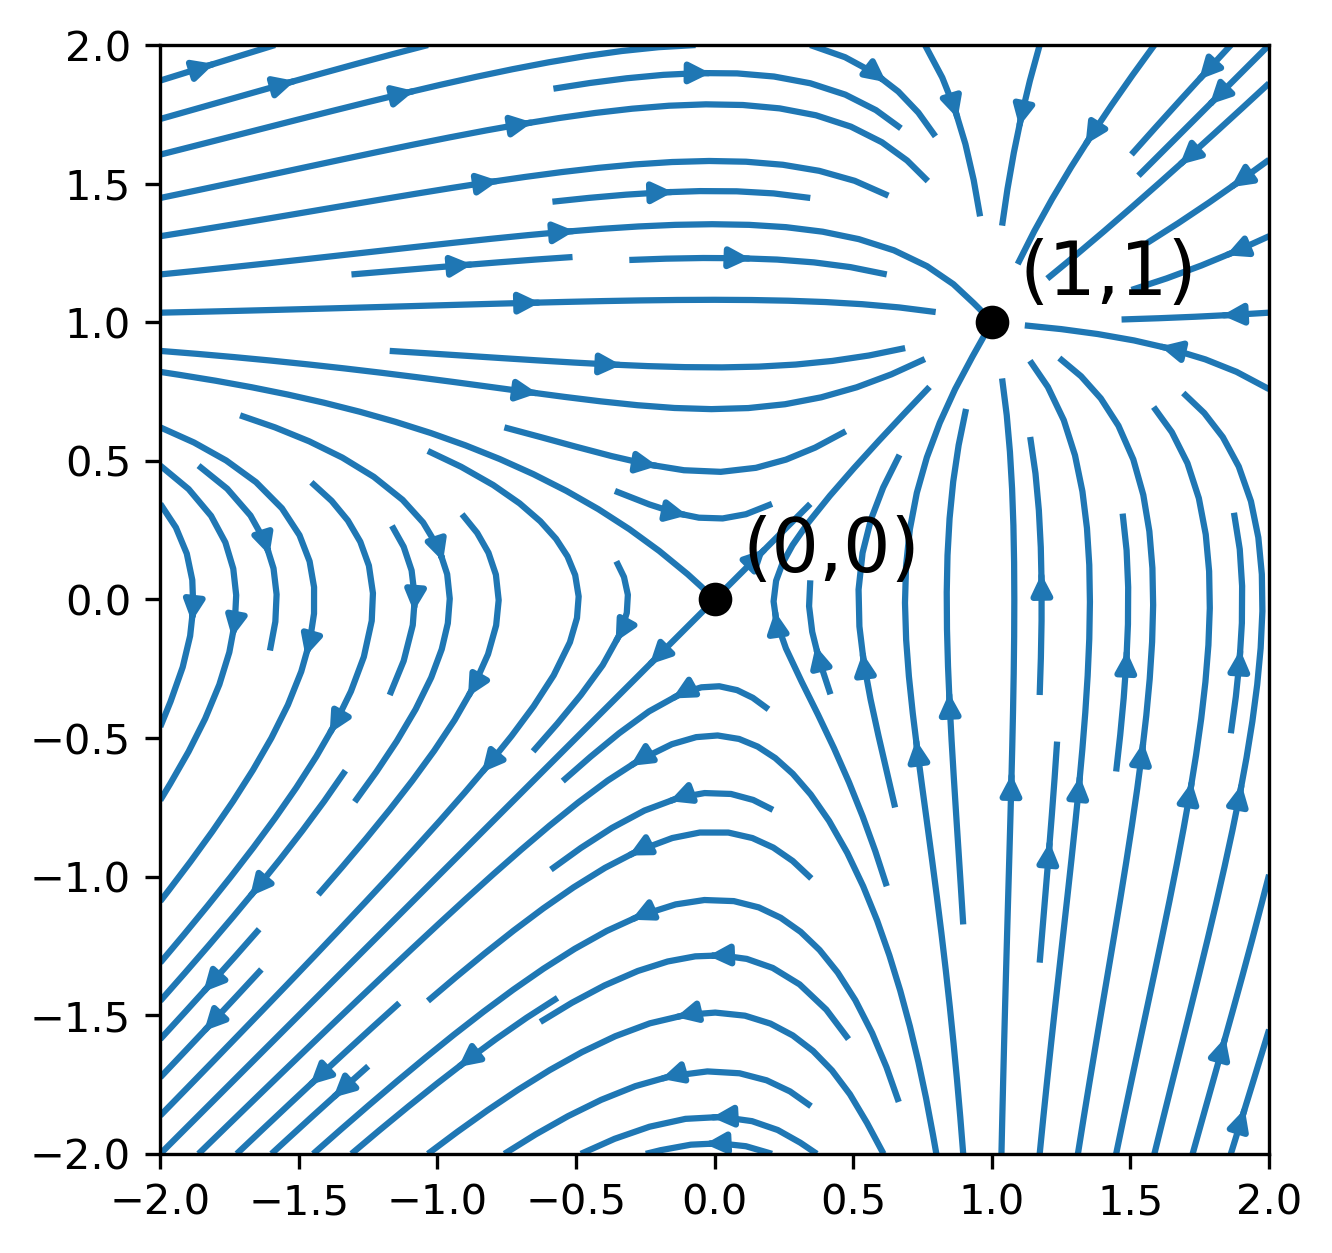
\includegraphics[scale=0.7]{graphics/saddlenode.png}
    \caption{\textit{The stream plot for the dynamical system in Example \ref{exmp:nonlindynsaddlenode}.}}
    \label{fig:nonlinearphase}
\end{figure}

\section{Earth Science Applications: the Lorenz-63 Model}

The \index{Lorenz-63 Model}\keywordhl{Lorenz-63 Model} is consisted of three variables $X,Y,Z$ and their evolutions in time are described by
\begin{subequations}
\label{eqn:lor63f}
\begin{empheq}[left={\empheqlbrace}]{alignat=1}
\frac{dX}{dt} &= -\sigma X + \sigma Y \label{eqn:lor63a} \\ 
\frac{dY}{dt} &= -XZ + \rho X - Y \label{eqn:lor63b} \\
\frac{dZ}{dt} &= XY - \beta Z \label{eqn:lor63c}
\end{empheq}
\end{subequations}
where the parameters $\sigma, \rho, \beta > 0$ are all positive. It is a minimalist model that demonstrates the phenomenon of \textit{chaos}. In the following subsections, we will discuss the context in which the model is formulated and the characteristics of its equilibrium points.

\subsection{Derivation of the Lorenz-63 Model}

\textit{Reference Materials: \cite{kaic}}

The Lorenz-63 model originates from a simplified version of the \index{Rayleigh-Barnard Convection}\textit{Rayleigh-Barnard Convection} problem about the convective/diffusion-driven flow. Particularly, we will restrict ourselves to a two-dimensional flow in the $x$/$z$-(zonal/meridional) directions so that the velocity vector is $\vec{u} = (u_x, 0, u_z)^T$. The governing equations for this scenario are the zonal/meridional \textit{momentum equations}, \textit{thermodynamics equation}, and the \textit{continuity equation} with \textit{Boussinesq approximation} as follows. \begin{empheq}[left={\empheqlbrace}]{alignat=2}
& \frac{\partial u_x}{\partial t} + u_x\frac{\partial u_x}{\partial x} + u_z \frac{\partial u_x}{\partial z} & &= \nu(\frac{\partial^2 u_x}{\partial x^2} + \frac{\partial^2 u_x}{\partial z^2}) - \frac{1}{\rho_0} \frac{\partial p}{\partial x} \label{eqn:RB1} \\
&\frac{\partial u_z}{\partial t} + u_x\frac{\partial u_z}{\partial x} + u_z \frac{\partial u_z}{\partial z} & &= \nu(\frac{\partial^2 u_z}{\partial x^2} + \frac{\partial^2 u_z}{\partial z^2}) - \frac{1}{\rho_0} \frac{\partial p}{\partial z} + \alpha T g \label{eqn:RB2} \\
&\frac{\partial T}{\partial t} - u_z\Gamma + u_x\frac{\partial T}{\partial x} + u_z\frac{\partial T}{\partial z} & &= \kappa (\frac{\partial^2 T}{\partial x^2} + \frac{\partial^2 T}{\partial z^2})  \label{eqn:RB3} \\
& \frac{\partial u_x}{\partial x} + \frac{\partial u_z}{\partial z} & &= 0 \label{eqn:RB4}
\end{empheq}
The constants are: $g$, the gravitational acceleration; $\alpha$, the thermal expansion coefficient of the fluid; the lapse rate $\Gamma = -\frac{T_H - T_L}{d}$ which is the difference in the temperature prescribed at the top and bottom plates over the vertical depth of the fluid $d$; $\rho_0$, the reference fluid density; $\nu$ and $\kappa$, the kinematic viscosity and thermal diffusivity. In addition to the velocities $u_x$ and $u_z$, there are two other variables: $T$ as the departure of temperature from the reference profile and $p$ as the pressure perturbation. By the \index{Buckingham Pi Theorem}\keywordhl{Buckingham Pi Theorem}\footnote{It states that all physically consistent laws are "unit-independent" and the number of non-dimensional variables required to transform a set of equations into dimensionless form is the number of physical variables minus the number of fundamental physical dimensions. There are $13$ physical variables here, time $t$, two displacements $x$ and $z$, two velocities $u_x$ and $u_z$, temperature $T$, kinematic viscosity $\nu$, thermal diffusivity $\kappa$, pressure $p$, density $\rho_0$, thermal expansion coefficient $\alpha$ and gravity $g$ (together counted as a single variable as they appear in the equation once and only once in combination over the term $\alpha Tg$), and finally two other variables, the vertical depth $d$ and temperature difference $T_H-T_L$ (derived from lapse rate $\Gamma$). Meanwhile, there are $4$ fundamental dimensions: length, time, mass, and temperature. So there will be $13 - 4 = 9$ non-dimensional variables.}, we can convert these equations into dimensionless form using $9$ non-dimensional variables:
\begin{subequations}
\begin{empheq}[left={\empheqlbrace}]{alignat=2}
&x^* & &= \frac{x}{d}\\
&z^* & &= \frac{z}{d}\\
&t^* & &= \frac{t}{d^2/\kappa}\\
&u_x^* & &= \frac{u_x}{\kappa/d}\\
&u_z^* & &= \frac{u_z}{\kappa/d}\\
&T^* & &= \frac{T}{\kappa\nu/g\alpha d^3}\\
&p^* & &= \frac{p}{\rho_0\kappa^2/d^2}\\
&\sigma & &= \frac{\nu}{\kappa}\\
&R & &= \frac{g\alpha d^3(T_H-T_L)}{\kappa\nu}
\end{empheq}
\end{subequations}
The first $7$ of them are the non-dimensional (indicated by the asterisk $^*$) physical variables of displacements, time, velocities, temperature, and pressure with the characteristic length/time/velocity/temperature/pressure scales of $d$, $d^2/\kappa$ (the \textit{dissipation timescale}), $\kappa/d$, $\kappa\nu/g\alpha d^3$, and $\rho_0\kappa^2/d^2$. The last two of them are the \index{Prandlt number}\textit{Prandlt Number} $\sigma = \frac{\nu}{\kappa}$ as the ratio of kinematic viscosity $\nu$ to thermal diffusivity $\kappa$, and \index{Rayleigh Number} \textit{Rayleigh number} \smash{$R = \frac{g\alpha d^3(T_H-T_L)}{\kappa\nu}$}. As we will see later, these two parameters will decide the behavior of the system. By substituting all these into (\ref{eqn:RB1}), we have
\begin{align*}
&\quad \left(\frac{\kappa/d}{d^2/\kappa}\right)\frac{\partial u_x^*}{\partial t^*} + \left(\frac{(\kappa/d)^2}{d}\right)u_x^*\frac{\partial u_x^*}{\partial x^*} + \left(\frac{(\kappa/d)^2}{d}\right)u_z^* \frac{\partial u_x^*}{\partial z^*} \\
&= \nu\left(\left(\frac{\kappa/d}{d^2}\right)\frac{\partial^2 u_x^*}{\partial {x^*}^2} + \left(\frac{\kappa/d}{d^2}\right)\frac{\partial^2 u_x^*}{\partial {z^*}^2}\right) - \left(\frac{\kappa^2/d^2}{d}\right)\frac{\partial p^*}{\partial x^*}    
\end{align*}
Dividing both sides of the equation by the factor \smash{$\frac{\kappa^2}{d^3}$} leads to
\begin{align}
\frac{\partial u_x^*}{\partial t^*} + u_x^*\frac{\partial u_x^*}{\partial x^*} + u_z^* \frac{\partial u_x^*}{\partial z^*} 
&= \frac{\nu}{\kappa}\left(\frac{\partial^2 u_x^*}{\partial {x^*}^2} + \frac{\partial^2 u_x^*}{\partial {z^*}^2}\right) - \frac{\partial p^*}{\partial x^*} \nonumber \\
&= \sigma\left(\frac{\partial^2 u_x^*}{\partial {x^*}^2} + \frac{\partial^2 u_x^*}{\partial {z^*}^2}\right) - \frac{\partial p^*}{\partial x^*} \label{eqn:RB1n}
\end{align}
Similarly, by noticing that $\alpha T g = \frac{\kappa\nu}{d^3} T^*$, we can rewrite (\ref{eqn:RB2}) into
\begin{align}
\frac{\partial u_z^*}{\partial t^*} + u_x^*\frac{\partial u_z^*}{\partial x^*} + u_z^* \frac{\partial u_z^*}{\partial z^*} &= \sigma\left(\frac{\partial^2 u_z^*}{\partial {x^*}^2} + \frac{\partial^2 u_z^*}{\partial {z^*}^2}\right) - \frac{\partial p^*}{\partial z^*} + \sigma T^* \label{eqn:RB2n}
\end{align}
Meanwhile, (\ref{eqn:RB3}) can be transformed into
\begin{align*}
&\quad \left(\frac{\kappa\nu/g\alpha d^3}{d^2/\kappa}\right)\frac{\partial T^*}{\partial t^*} + (\kappa/d)u_z^* \left(\frac{T_L - T_H}{d}\right) \\
&\quad + \left(\frac{(\kappa/d)(\kappa\nu/g\alpha d^3)}{d}\right)u_x^*\frac{\partial T^*}{\partial x^*} + \left(\frac{(\kappa/d)(\kappa\nu/g\alpha d^3)}{d}\right)u_z^*\frac{\partial T^*}{\partial z^*} \\
&= \kappa \left(\left(\frac{\kappa\nu/g\alpha d^3}{d^2}\right)\frac{\partial^2 T^*}{\partial {x^*}^2} + \left(\frac{\kappa\nu/g\alpha d^3}{d^2}\right)\frac{\partial^2 T^*}{\partial {z^*}^2}\right)  
\end{align*}
This time, dividing by the factor \smash{$\frac{\kappa^2\nu}{g\alpha d^5}$} gives
\begin{align}
&\quad \frac{\partial T^*}{\partial t^*} + u_z^* \left(\frac{g\alpha d^3(T_H - T_L)}{\kappa\nu}\right) + u_x^*\frac{\partial T^*}{\partial x^*} + u_z^*\frac{\partial T^*}{\partial z^*} \nonumber \\
&= \frac{\partial T^*}{\partial t^*} + R u_z^* + u_x^*\frac{\partial T^*}{\partial x^*} + u_z^*\frac{\partial T^*}{\partial z^*} = \frac{\partial^2 T^*}{\partial {x^*}^2} + \frac{\partial^2 T^*}{\partial {z^*}^2} \label{eqn:RB3n}
\end{align}
Finally, the non-dimensional form of the mass continuity equation (\ref{eqn:RB4}) is simply
\begin{align}
\frac{\partial u_x^*}{\partial x^*} + \frac{\partial u_z^*}{\partial z^*} &= 0 \label{eqn:loreznmasscont}
\end{align}
According to this, we can rewrite $\vec{u}^* = (u_x^*, 0, u_z^*)^T = (-\frac{\partial \psi^*}{\partial z^*}, 0, \frac{\partial \psi^*}{\partial x^*})$ where $\psi^*$ is known as the (non-dimensional) \index{Stream Function}\keywordhl{stream function}. This is possible as the problem is set up to be two-dimensional and we will further require it to be bounded, such that $\vec{u} = \textbf{0}$ and $T = 0$ ($\vec{u}^* = \textbf{0}$ and $T^* = 0$) at $z = 0,d$ ($z^* = 0,1$) and the boundary condition along the $x$-direction is periodic. With
\begin{subequations}
\label{eqn:lorenzstreamv}
\begin{empheq}[left={\empheqlbrace}]{alignat=1}
u_x^* &= -\frac{\partial \psi^*}{\partial z^*} \\
u_z^* &= \frac{\partial \psi^*}{\partial x^*}
\end{empheq}
\end{subequations}
(\ref{eqn:loreznmasscont}) is then automatically satisfied.\footnote{$\frac{\partial u_x^*}{\partial x^*} + \frac{\partial u_z^*}{\partial z^*} = -\frac{\partial \psi^*}{\partial x^*\partial z^*} + \frac{\partial \psi^*}{\partial x^*\partial z^*} \equiv 0$.} Now substituting (\ref{eqn:lorenzstreamv}) into (\ref{eqn:RB1n}) and (\ref{eqn:RB2n}), and writing $\frac{\partial}{\partial[\;]} = \partial_{[\;]}$ for simplicity, we have
\begin{align}
&\quad \partial_{t^*} \partial_{z^*} \psi^* - (\partial_{z^*} \psi^*)(\partial_{x^*} \partial_{z^*} \psi^*) + (\partial_{x^*} \psi^*) ((\partial_{z^*})^2 \psi^*) \nonumber \\
&= \sigma\left((\partial_{x^*})^2\partial_{z^*} \psi^* + (\partial_{z^*})^3 \psi^* \right) + \partial_{x^*} p^* \label{eqn:RBpsia}
\end{align}
and
\begin{align}
&\quad \partial_{t^*} \partial_{x^*} \psi^* - (\partial_{z^*} \psi^*)((\partial_{x^*})^2 \psi^*) + (\partial_{x^*} \psi^*) (\partial_{z^*} \partial_{x^*} \psi^*) \nonumber \\
&= \sigma\left((\partial_{x^*})^3 \psi^* + (\partial_{z^*})^2 \partial_{x^*} \psi^* \right) - \partial_{z^*} p^* + \sigma T^* \label{eqn:RBpsib}
\end{align}
Differentiating (\ref{eqn:RBpsia}) with respect to $z$ and (\ref{eqn:RBpsib}) with respect to $x$, and then adding them together will eliminate the pressure term and lead to an L.H.S. of
\begin{align*}
&\quad [\partial_{t^*}  (\partial_{z^*} )^2 \psi^* \mathcolor{red}{-((\partial_{z^*} )^2 \psi^*)(\partial_{x^*}  \partial_{z^*}  \psi^*)}  - (\partial_{z^*}  \psi^*)(\partial_{x^*}  (\partial_{z^*} )^2 \psi^*) \\
&\quad \mathcolor{red}{+ (\partial_{z^*}  \partial_{x^*}  \psi^*) ((\partial_{z^*} )^2 \psi^*)} + (\partial_{x^*}  \psi^*) ((\partial_{z^*} )^3 \psi^*)] \\
&\quad + [\partial_{t^*}  (\partial_{x^*} )^2 \psi^* \mathcolor{red}{- (\partial_{x^*} \partial_{z^*}  \psi^*)((\partial_{x^*} )^2 \psi^*)} - (\partial_{z^*}  \psi^*)((\partial_{x^*} )^3 \psi^*) \\
&\quad \mathcolor{red}{+ ((\partial_{x^*} )^2 \psi^*) (\partial_{z^*}  \partial_{x^*}  \psi^*)} + (\partial_{x^*}  \psi^*) (\partial_{z^*}  (\partial_{x^*} )^2 \psi^*)] \\
&= \partial_{t^*}  \left((\partial_{x^*} )^2 + (\partial_{z^*})^2\right) \psi^* - (\partial_{z^*} \psi^*) (\partial_{x^*}  \left((\partial_{x^*})^2 + (\partial_{z^*})^2\right)\psi^*) \\
&\quad + (\partial_{x^*} \psi^*) (\partial_{z^*} \left((\partial_{x^*})^2 + (\partial_{z^*})^2\right)\psi^*) 
\end{align*}
and an R.H.S. of
\begin{align*}
&\quad [\sigma\left((\partial_{x^*})^2(\partial_{z^*})^2 \psi^* + (\partial_{z^*})^4 \psi^* \right) \mathcolor{red}{+ \partial_{z^*} \partial_{x^*} p^*}] \\
&\quad + [\sigma\left((\partial_{x^*})^4 \psi^* + (\partial_{z^*})^2 (\partial_{x^*})^2 \psi^* \right) \mathcolor{red}{- \partial_{x^*} \partial_{z^*} p^*} + \sigma \partial_{x^*} T^*] \\
&= \sigma \left((\partial_{x^*})^2 + (\partial_{z^*})^2\right)^2 \psi^* + \sigma \partial_{x^*} T^*
\end{align*}
By using the \index{Laplacian}\textit{Laplacian} symbol $\Delta^* = (\partial_{x^*})^2 + (\partial_{z^*})^2$ in this equation, and also substituting the stream function (\ref{eqn:lorenzstreamv}) into the other equation (\ref{eqn:RB3n}), we can sort out a set of two equations in two unknowns $\psi^*$ and $T^*$, that describes the evolution of the system state:
\begin{empheq}[left={\empheqlbrace}]{alignat=1}
\partial_{t^*} \Delta^* \psi^* - (\partial_{z^*} \psi^*) (\partial_{x^*}\Delta^* \psi^*) + (\partial_{x^*} \psi^*) (\partial_{z^*}\Delta^* \psi^*) &= \sigma {\Delta^*}^2\psi^* + \mathrlap{\sigma \partial_{x^*} T^*} \label{eqn:lorenzwind} \\
\partial_{t^*}T^* - (\partial_{z^*} \psi^*)(\partial_{x^*} T^*) + (\partial_{x^*} \psi^*)(\partial_{z^*} T^*) &= \Delta^* T^* - R \partial_{x^*} \psi^* \label{eqn:lorenztemp}
\end{empheq} As mentioned before, the statistics of the system are controlled by the two parameters $\sigma$ and $R$ here. However, we still have to simplify the problem to make it tractable while retaining the chaotic nature. For this, we will decompose the variables $T^*$ and $\psi^*$ into Fourier modes along the zonal and meridional directions. Since the boundary conditions are periodic and fixed to zero in the $x$ and $z$-directions respectively, we assume that the solution will take the following form of infinite summations of basis functions in terms of products between complex exponentials and sines (can refer to Section \ref{section:DFT}):
\begin{subequations}
\begin{empheq}[left={\empheqlbrace}]{alignat=1}
T^*(x^*,z^*,t^*) &= \sum_{k_1 = -\infty}^{\infty} \sum_{k_2 = 1}^{\infty} \hat{T}_{k_1,k_2}(t^*) e^{ik_1\pi a x^*} \sin(k_2\pi z^*) \\
\psi^*(x^*,z^*,t^*) &= \sum_{k_1 = -\infty}^{\infty} \sum_{k_2 = 1}^{\infty} \hat{\psi}_{k_1,k_2}(t^*) e^{ik_1\pi a x^*} \sin(k_2\pi z^*)
\end{empheq}     
\end{subequations}
where $a = d/l$ is the aspect ratio (depth to width) of the domain\footnote{$\frac{z}{d} = z^*$, $\frac{x}{l} = \frac{dx^*}{l} = ax^*$.}. To proceed, we first need to understand that to generate various Fourier basis functions with new wave numbers, we have to rely on the non-linearity due to the interaction of flow with different wave numbers (scales). Otherwise, the orthogonality of the Fourier modes will prevent this from happening over linear terms. Heuristically, if we look at, for example, the portion of the complex exponentials in $x^*$ for two $\psi^*$ basis functions, \smash{$\hat{\psi}_{k} e^{ik\pi a x^*}$} and \smash{$\hat{\psi}_{l} e^{il\pi a x^*}$}, then their product (as well as with one of them conjugated) will produce
\begin{subequations}
\label{eqn:nonlinearinter}
\begin{empheq}[left={\empheqlbrace}]{alignat=1}
\psi^*_k\psi^*_l &= \hat{\psi}_{k}\hat{\psi}_{l} e^{i(k+l)\pi a x^*} \\
\psi^*_k\overline{\psi^*_l} &= \hat{\psi}_{k}\overline{\hat{\psi}_{l}} e^{i(k-l)\pi a x^*}
\end{empheq} 
\end{subequations}
So the new signal can have either a wave number of $k + l$ and $k - l$. If particularly one of the original wave numbers $k$ and $l$ is $1$, then by inductively using this property we can essentially generate all wave numbers and hence the full dynamics. Therefore, we are motivated to focus on the Fourier modes with a wave number of $1$. Again we will first look at the $x^*$ portion of the Fourier modes and we will choose the imaginary part of $\hat{\psi}_{k_1 = 1}$ which is $\hat{\psi}_{k_1 = 1} \sin(\pi a x^*)$ as the starting point. We will drop the non-linear advection term $- (\partial_{z^*} \psi^*) (\partial_{x^*}\Delta^* \psi^*) + (\partial_{x^*} \psi^*) (\partial_{z^*}\Delta^* \psi^*)$ in the prognostic equation (\ref{eqn:lorenzwind}) of $\psi^*$ to trim down the model. This makes the $\sigma \partial_{x^*} T^*$ term on R.H.S. become the only way to keep the non-linearity (the remaining $\sigma {\Delta^*}^2\psi^*$ is only a linear damping term). For this $\sigma \partial_{x^*} T^*$ term to contribute to the tendency of $\hat{\psi}_{k_1 = 1} \sin(\pi a x^*)$ in the time derivative term $\partial_{t^*} \Delta^* \psi^*$ on L.H.S., we must also have the real part of $\hat{T}_{k_1 = 1}$ which is $\hat{T}_{k_1 = 1} \cos(\pi a x^*)$, due to the form of $\sigma \partial_{x^*} T^*$ which upon substitution becomes $-\sigma \pi a \hat{T}_{k_1 = 1} \sin(\pi a x^*)$, so that it is compatible with the sine part of $\hat{\psi}_{k_1 = 1} \sin(\pi a x^*)$ with a wave number of $1$. \par

Since we have removed the advection term in the prognostic equation of $\psi^*$, we have to keep the advection term $- (\partial_{z^*} \psi^*)(\partial_{x^*} T^*) + (\partial_{x^*} \psi^*)(\partial_{z^*} T^*)$ in the prognostic equation of $T^*$ to ensure the non-linearity of the whole dynamical system. By the previous argument over (\ref{eqn:nonlinearinter}), as long as either the sum of or difference in wave numbers $k_1$ and $k_2$ between the two scales is $1$ ($k_1 + k_2 = 1$ or $k_1 - k_2 = 1$), then their non-linear interaction can generate the required wave number $1$ signal (the real part of $\hat{T}_{k_1 = 1}$). One of the simplest ways to achieve this without involving too many new scales is to introduce the real part of the mean temperature $\hat{T}_{k_1 = 0}$ which is a constant in $x^*$, so that the forcing term for $\hat{T}_{k_1 = 1} \cos(\pi ax^*)$ is produced in (\ref{eqn:lorenztemp}) as we already have $\hat{\psi}_{k_1 = 1}$. Physically, it represents the non-linear interaction between the mean temperature field and the zonal wave number 1 flow. So we come to the third variable $\hat{T}_{k_1 = 0}$ finally. To verify if we can close the equations so that there are enough forcing terms for all three included wave numbers, we can check if the non-linear interaction between the imaginary part of $\hat{\psi}_{k_1 = 1}$ and the real part of $\hat{T}_{k_1 = 1}$ indeed brings us $\hat{T}_{k_1 = 0}$. Substituting the relevant expressions into the advection term $-(\partial_{z^*} \psi^*)(\partial_{x^*} T^*) + (\partial_{x^*} \psi^*)(\partial_{z^*} T^*)$ in (\ref{eqn:lorenztemp}), we have (where we can ignore any part related to $z^*$ for now)
\begin{align*}
&\quad -(\partial_{z^*} \psi^*)(\partial_{x^*} T^*) + (\partial_{x^*} \psi^*)(\partial_{z^*} T^*) \\
&= -\hat{\psi}_{k_1 = 1} \sin(\pi a x^*) \partial_{x^*} (\hat{T}_{k_1 = 1} \cos(\pi a x^*)) \\
&\quad + \partial_{x^*}(\hat{\psi}_{k_1 = 1} \sin(\pi a x^*))\hat{T}_{k_1 = 1} \cos(\pi a x^*) \\
&= -\hat{\psi}_{k_1 = 1} \sin(\pi a x^*)(-\pi a\hat{T}_{k_1 = 1}\sin(\pi a x^*)) \\
&\quad + (\pi a\hat{\psi}_{k_1 = 1}\cos(\pi a x^*)) \hat{T}_{k_1 = 1} \cos(\pi a x^*) \\
&= \pi a \hat{\psi}_{k_1 = 1}\hat{T}_{k_1 = 1}(\sin^2(\pi a x^*) + \cos^2(\pi a x^*)) = \pi a \hat{\psi}_{k_1 = 1}\hat{T}_{k_1 = 1}
\end{align*}
which indeed gives the zonally constant temperature forcing as desired. We repeat the same analysis for the $z$ portion of the Fourier modes and similarly start with  $\hat{\psi}_{k_2 = 1}\sin(\pi z^*)$ and $\hat{T}_{k_2 = 1} \sin(\pi z^*)$ of the same wave numbers. This time we will need the meridional wave number $2$ temperature field and we will check following the same logic above:
\begin{align*}
&\quad -(\partial_{z^*} \psi^*)(\partial_{x^*} T^*) + (\partial_{x^*} \psi^*)(\partial_{z^*} T^*) \\
&= -(\pi\hat{\psi}_{k_2 = 1}\cos(\pi z^*)) (\mathcolor{red}{(-)}\hat{T}_{k_2 = 1} \sin(\pi z^*)) \\
&\quad + \hat{\psi}_{k_2 = 1}\sin(\pi z^*) (\pi\hat{T}_{k_2 = 1} \cos(\pi z^*)) \\
&\quad
\begin{aligned}
&\textcolor{red}{\text{(Notice that the differentiation of the real part of $\hat{T}_{k_1 = 1}$ with respect to $x$}} \\
&\textcolor{red}{\text{in the first term will contribute an extra negative sign as above)}}
\end{aligned} \\
&= 2\pi\hat{\psi}_{k_2 = 1}\hat{T}_{k_2 = 1} \sin(\pi z^*)\cos(\pi z^*) = \pi\hat{\psi}_{k_2 = 1}\hat{T}_{k_2 = 1} \sin(2\pi z^*)
\end{align*}
Now we will combine all of these where the needed three variables are the imaginary part of $\smash{\hat{\psi}_{k_1 = 1, k_2 = 1}}$, and the real parts of $\smash{\hat{T}_{k_1 = 1, k_2 = 1}}$ and $\smash{\hat{T}_{k_1 = 0, k_2 = 2}}$ respectively. Substituting them into (\ref{eqn:lorenzwind}), we have
\begin{align}
&\quad \partial_{t^*} \Delta^* (\hat{\psi}_{k_1 = 1, k_2 = 1}\sin(\pi a x^*)\sin(\pi z^*)) \nonumber \\
&= \sigma {\Delta^*}^2 (\hat{\psi}_{k_1 = 1, k_2 = 1}\sin(\pi a x^*)\sin(\pi z^*))\nonumber \\
&\quad + \sigma \partial_{x^*} ((\hat{T}_{k_1 = 1, k_2 = 1}\cos(\pi a x^*)\sin(\pi z^*)) + (\hat{T}_{k_1 = 0, k_2 = 2}\sin(2\pi z^*))) \nonumber \\
\nonumber \\
\implies &\quad -\partial_{t^*}(\hat{\psi}_{k_1 = 1, k_2 = 1}\sin(\pi a x^*)\sin(\pi z^*)) \nonumber \\
&= \sigma (\hat{\psi}_{k_1 = 1, k_2 = 1}\sin(\pi a x^*)\sin(\pi z^*)) - \sigma (\hat{T}_{k_1 = 1, k_2 = 1}\sin(\pi a x^*)\sin(\pi z^*)) \nonumber \\
\implies &\quad \partial_{t^*}\hat{\psi}_{k_1 = 1, k_2 = 1} = \sigma\hat{T}_{k_1 = 1, k_2 = 1} - \sigma\hat{\psi}_{k_1 = 1, k_2 = 1} 
\end{align}
where we have ignored any scaling constant arising from differentiation except the negative sign, and the only effect of the Laplacian $\Delta$ is hence to introduce an extra negative sign.\footnote{To illustrate, $\Delta^*((\sin(\pi a x^*)\sin(\pi z^*)) = ((\partial_{x^*})^2 + (\partial_{z^*})^2)((\sin(\pi a x^*)\sin(\pi z^*)) = -\pi^2a^2 (\sin(\pi a x^*)\sin(\pi z^*)) - \pi^2 (\sin(\pi a x^*)\sin(\pi z^*)) = -(\pi^2a^2 + \pi^2)(\sin(\pi a x^*)\sin(\pi z^*))$.} Replacing $\hat{\psi}_{k_1 = 1, k_2 = 1}, \hat{T}_{k_1 = 1, k_2 = 1}, \hat{T}_{k_1 = 0, k_2 = 2}$ by $X$, $Y$, $Z$ respectively then readily yields (\ref{eqn:lor63a}). In the same essence, we can derive the other two equations (\ref{eqn:lor63b}) and (\ref{eqn:lor63c}) of the Lorenz-63 Model by substitution into (\ref{eqn:lorenztemp}) with some adjustments to the parameters.\footnote{Unfortunately, the algebra is too tedious to be included in the text. Any ambitious reader can try it though.} Now the $\rho$ in (\ref{eqn:lor63b}) represents a rescaling of the Rayleigh number relative to the \textit{critical} Rayleigh number which dictates the initialization of the convection and $\beta$ in (\ref{eqn:lor63c}) comes from the aspect ratio. With (\ref{eqn:lor63f}) derived properly, we are ready to examine the nature of its dynamics.

\subsection{Stability Analysis of Each Equilibrium Point}

\textit{Reference Materials: \cite{lorenz}}

We will inspect the stability of each equilibrium point of the Lorenz-63 Model and thus its behavior under different parameter settings. First, from (\ref{eqn:lor63f}) it is obvious that the origin $\textbf{0} = (0,0,0)^T$ is an equilibrium point. The other equilibrium points can be found by first noticing that (\ref{eqn:lor63a}) requires $\tilde{X}=\tilde{Y}$. Substituting this into (\ref{eqn:lor63b}) and (\ref{eqn:lor63c}) gives
\begin{empheq}[left={\empheqlbrace}]{alignat=1}
-\tilde{X}\tilde{Z} + \rho \tilde{X} - \tilde{X} &= 0 \implies \tilde{Z} = \rho - 1 \nonumber \\
\tilde{X}^2 - \beta \tilde{Z} &= 0 \nonumber
\end{empheq}
Combining these two equations leads to
\begin{align*}
\tilde{X}^2 = \beta (\rho - 1) \implies \tilde{X} = \pm\sqrt{\beta (\rho - 1)}
\end{align*}
Therefore the other two equilibrium points are
\begin{align}
\tilde{\textbf{X}}_{\pm} = (\pm\sqrt{\beta (\rho - 1)}, \pm\sqrt{\beta (\rho - 1)}, \rho-1)^T \label{eqn:paireqptslorenz}
\end{align}
which only emerge when $\rho > 1$ due to the square roots in the $X$ and $Y$ components. Therefore, we can divide the system into two major cases: $0 < \rho < 1$ and $\rho > 1$.\footnote{$\rho = 1$, as well as $\rho = \rho_c$ that we will see later, belongs to the special case of a \textit{bifurcation point} where transition happens and their treatment is out of the scope of this book.} When $0 < \rho < 1$, the origin is the only equilibrium point. According to (\ref{eqn:nonlindynjac})), the linearized system will have a Jacobian of
\begin{align}
\frac{\partial F_i}{\partial X_j} =
\begin{bmatrix}
\dfrac{\partial F_1}{\partial X} & \dfrac{\partial F_1}{\partial Y} & \dfrac{\partial F_1}{\partial Z} \\[10pt]
\dfrac{\partial F_2}{\partial X} & \dfrac{\partial F_2}{\partial Y} & \dfrac{\partial F_2}{\partial Z} \\[10pt]
\dfrac{\partial F_3}{\partial X} & \dfrac{\partial F_3}{\partial Y} & \dfrac{\partial F_3}{\partial Z}
\end{bmatrix}
=
\begin{bmatrix}
-\sigma & \sigma & 0 \\
\rho-Z & -1 & -X \\
Y & X & -\beta
\end{bmatrix}
\label{eqn:lorenzjac}
\end{align}
At the origin, it is
\begin{align}
\left.\frac{\partial F_i}{\partial X_j}\right|_{\textbf{0}} =
\begin{bmatrix}
-\sigma & \sigma & 0 \\
\rho & -1 & 0 \\
0 & 0 & -\beta
\end{bmatrix}
\end{align}
the characteristic polynomial of which is
\begin{align}
\det(\left.\frac{\partial F_i}{\partial X_j}\right|_{\textbf{0}} - \lambda I) &= 
\begin{vmatrix}
-\sigma-\lambda & \sigma & 0 \\
\rho & -1-\lambda & 0 \\
0 & 0 & -\beta-\lambda
\end{vmatrix} \nonumber \\
&= -(\lambda + \beta)((-\sigma-\lambda)(-1-\lambda) - \rho\sigma) \nonumber \\
&= -(\lambda + \beta)(\lambda^2 + (1+\sigma)\lambda - (\rho-1)\sigma)
\end{align}
The roots are $\lambda_1 = -\beta$ and
\begin{align}
\lambda_{\pm} &= \frac{1}{2}\left(-(1+\sigma) \pm \sqrt{(1+\sigma)^2 - (-4(\rho-1)\sigma)}\right) \nonumber \\
&= \frac{1}{2}\left(-(1+\sigma) \pm \sqrt{(1+\sigma)^2 + (4\rho\sigma-4\sigma)}\right) = \frac{1}{2}(-(1+\sigma) \pm \sqrt{\mathcal{D}})
\end{align}
by the quadratic equation formula where $\mathcal{D}$ denotes the discriminant. When $0 < \rho < 1$, 
\begin{align*}
\sqrt{\mathcal{D}} &= \sqrt{(1+\sigma)^2 + (4\rho\sigma-4\sigma)} \\
&< \sqrt{(1+\sigma)^2} = 1+\sigma
\end{align*}
and therefore the two other roots $\lambda_{\pm} = \frac{1}{2}(-(1+\sigma) \pm \sqrt{\mathcal{D}}) < 0$ must also be negative. By the Hartman-Grobman Theorem \ref{thm:HGthm}, the origin is hence a hyperbolic equilibrium point which is locally a stable node. Therefore, when $0 < \rho < 1$, the entire Lorenz-63 Model is stable, which corresponds to the physical situation where the Rayleigh number does not reach the critical threshold and convection does not arise. However, when $\rho > 1$, by the same logic, now $\sqrt{D} > 1 + \sigma$ and one of the roots $\lambda_{+} > 0$ will be positive, and the origin then becomes a saddle point. At the same time, as $\rho > 1$, there will appear two new equilibrium points indicated by (\ref{eqn:paireqptslorenz}) and we are going to determine their types as well. However, it is instructive to first note that we only need to consider either of them because the Lorenz-63 Model itself, in addition to these two equilibrium points, is symmetric in the $X$ and $Y$ directions.\footnote{Replacing $X$ by $-X$ and $Y$ by $-Y$ in (\ref{eqn:lor63f}) gives
\begin{empheq}[left={\empheqlbrace}]{alignat=2}
\frac{d(-X)}{dt} &= -\sigma (-X) + \sigma (-Y) &\implies \frac{dX}{dt} &= -\sigma X + \sigma Y \nonumber \\ 
\frac{d(-Y)}{dt} &= -(-X)Z + \rho (-X) - (-Y) &\implies \frac{dY}{dt} &= -XZ + \rho X - Y \nonumber \\
\frac{dZ}{dt} &= (-X)(-Y) - \beta Z &\implies \frac{dZ}{dt} &= XY - \beta Z  \nonumber
\end{empheq}
which is exactly the same as (\ref{eqn:lor63f}).} We will take the positive equilibrium point $\tilde{\textbf{X}}_{+} = (\sqrt{\beta (\rho - 1)}, \sqrt{\beta (\rho - 1)}, \rho-1)^T$. The Jacobian of linearization at this equilibrium point is found by substituting it into (\ref{eqn:lorenzjac}), which gives
\begin{align}
\left.\frac{\partial F_i}{\partial X_j}\right|_{\tilde{\textbf{X}}_{+}} &=
\left[\begin{array}{@{\,}wc{50pt}wc{50pt}wc{55pt}@{\,}}
-\sigma & \sigma & 0 \\
\rho-(\rho - 1) & -1 & -\sqrt{\beta (\rho - 1)} \\
\sqrt{\beta (\rho - 1)} & \sqrt{\beta (\rho - 1)} & -\beta
\end{array}\right] \nonumber \\
&=
\left[\begin{array}{@{\,}wc{50pt}wc{50pt}wc{55pt}@{\,}}
-\sigma & \sigma & 0 \\
1 & -1 & -\sqrt{\beta (\rho - 1)} \\
\sqrt{\beta (\rho - 1)} & \sqrt{\beta (\rho - 1)} & -\beta
\end{array}\right]
\end{align}
and its characteristic polynomial is
\begin{align}
&\quad \det(\left.\frac{\partial F_i}{\partial X_j}\right|_{\tilde{\textbf{X}}_{+}} - \lambda I) \nonumber \\
&= 
\begin{vmatrix}
-\sigma-\lambda & \sigma & 0 \\
1 & -1-\lambda & -\sqrt{\beta (\rho - 1)} \\
\sqrt{\beta (\rho - 1)} & \sqrt{\beta (\rho - 1)} & -\beta-\lambda
\end{vmatrix} \nonumber \\ 
&= (-\sigma-\lambda)
\begin{vmatrix}
-1-\lambda & -\sqrt{\beta (\rho - 1)} \\  
\sqrt{\beta (\rho - 1)} & -\beta-\lambda 
\end{vmatrix} - \sigma
\begin{vmatrix}
1 & -\sqrt{\beta (\rho - 1)} \\
\sqrt{\beta (\rho - 1)} & -\beta-\lambda    
\end{vmatrix} \nonumber \\
&= (-\sigma - \lambda)((-1-\lambda)( -\beta-\lambda) - (\sqrt{\beta (\rho - 1)})(-\sqrt{\beta (\rho - 1)}) \nonumber \\
&\quad -\sigma((1)(-\beta-\lambda) - (\sqrt{\beta (\rho - 1)})(-\sqrt{\beta (\rho - 1)})) \nonumber \\
&= (-\sigma - \lambda)(\beta + (\beta+1)\lambda + \lambda^2 + \beta(\rho-1)) -\sigma(-\beta-\lambda + \beta (\rho - 1)) \nonumber\\
&= (-\sigma - \lambda)(\beta\rho + (\beta+1)\lambda + \lambda^2) + \beta\sigma + \sigma\lambda - \beta\sigma\rho + \beta\sigma \nonumber \\
&= (-\beta\sigma\rho -(\beta+1)\sigma\lambda - \sigma \lambda^2) + (-\beta\rho\lambda - (\beta+1)\lambda^2 - \lambda^3) \nonumber\\
&\quad + \beta\sigma + \sigma\lambda - \beta\sigma\rho + \beta\sigma \nonumber \\
&= -\lambda^3 - (\beta + \sigma + 1)\lambda^2 -\beta(\sigma + \rho)\lambda -2 \beta\sigma(\rho - 1) \label{eqn:lorenzcubicchar}
\end{align}
by Cofactor Expansion along the first row. As the coefficients of the characteristic polynomial are all negative as long as $\rho > 1$, the roots must be negative if they are real.\footnote{If any real root is positive, then $-\lambda^3 - (\beta + \sigma + 1)\lambda^2 -\beta(\sigma + \rho)\lambda - 2 \beta\sigma(\rho - 1) < 0 \neq 0$.} So the problem is reduced to determine the nature of its roots. Particularly, we are interested in the case when there are one real negative root and two complex roots, and the real part of the two complex roots changes from negative to positive. The required critical value of $\rho = \rho_c$ where this transition happens can be found by considering purely imaginary roots $\lambda = i\mu$ as the real part vanishes. Substituting this into (\ref{eqn:lorenzcubicchar}) gives
\begin{align}
&\quad -(i\mu)^3 - (\beta + \sigma + 1)(i\mu)^2 -\beta(\sigma + \rho_c)(i\mu) - 2 \beta\sigma(\rho_c - 1) \nonumber \\
&= i\mu^3 + (\beta + \sigma + 1)\mu^2 -i\beta(\sigma + \rho_c)\mu - 2 \beta\sigma(\rho_c - 1)
\end{align}
By equating real and imaginary parts, we have
\begin{subequations}
\begin{align}
(\beta + \sigma + 1)\mu^2 &= 2 \beta\sigma(\rho_c - 1) \\
\mu^3 &= \beta(\sigma + \rho_c)\mu 
\end{align}    
\end{subequations}
Combining these two equations (dividing (a) by (b)) then yields
\begin{align}
\beta + \sigma + 1 &= \frac{2 \beta\sigma(\rho_c - 1)}{\beta(\sigma + \rho_c)} \nonumber \\
(\beta + \sigma + 1)(\sigma + \rho_c) &= 2 \sigma(\rho_c - 1) \nonumber \\
\rho_c(\beta + \sigma + 1) + \sigma(\beta + \sigma + 1) &= 2 \sigma\rho_c - 2\sigma  \nonumber \\
\rho_c(\beta - \sigma + 1) &= -\sigma(\beta + \sigma + 3)  \nonumber \\
\rho_c &= \frac{\sigma(\beta + \sigma + 3)}{\sigma - \beta - 1} \label{eqn:lorezncrit}
\end{align}
However, this does not tell us which side, $\rho < \rho_c$ or $\rho > \rho_c$, corresponds to a positive/negative real part of the complex roots. We will simply state the conclusion for that.\footnote{Again, the algebra to explicitly show this is too horrifying to be written down.} If $\rho < \rho_c$, the complex roots will have a negative real part. So by the Hartman-Grobman Theorem \ref{thm:HGthm}, the equilibrium points $\tilde{\textbf{X}}_{\pm}$ will be stable, behaving as a one-dimensional manifold of a stable node and a two-dimensional manifold of a stable spiral combined together. Any particle will spiral inwards and be absorbed into either of the two equilibrium points. However, when $\rho > \rho_c$, the complex roots will now have a positive real part and by the same argument the equilibrium points $\tilde{\textbf{X}}_{\pm}$ will be unstable locally, akin to a one-dimensional manifold of a stable node fused with a two-dimensional manifold of an unstable spiral. The effect is to cause the particle to gradually spiral outwards about one of the equilibrium points, and when it moves far enough away from it, it will be attracted and gravitate towards the another equilibrium point. However, as the particle get closer to it, the same scenario will occur again where it will now gradually spiral outwards about the new equilibrium point. This alternating pattern will keep going on and on, where the particle will revolve about and be flung between these two equilibrium points. Hence, as $\rho > \rho_c$, the Lorenz-63 Model is known as a \index{Strange Attractor}\keywordhl{strange attractor} and \index{Chaos}\keywordhl{chaos} arises: the system is very sensitive to any small perturbation in the initial position of a particle and it can lead to great deviation in future trajectories (the \index{Butterfly Effect}\keywordhl{Butterfly Effect}). Physically, the Rayleigh number is sufficiently high to produce chaos. Usually, we set $\sigma = 10$ and $\beta = \frac{8}{3}$. The critical value of $\rho_c$ will then be
\begin{align}
\rho_c = \frac{(10)\left(\frac{8}{3} + 10 + 3\right)}{10 - \frac{8}{3} - 1} \approx 24.74
\end{align}
according to (\ref{eqn:lorezncrit}). The following two figures (Figures \ref{fig:lor63r14} and \ref{fig:lor63r28}) then show the evolution of the system with $\rho = 14$ and $\rho = 28$\footnote{$\rho = 28$ is a very common configuration picked to demonstrate the chaotic behavior.}, when $\rho$ is under and above the critical $\rho_c$.
\begin{figure}[p]
    \centering
    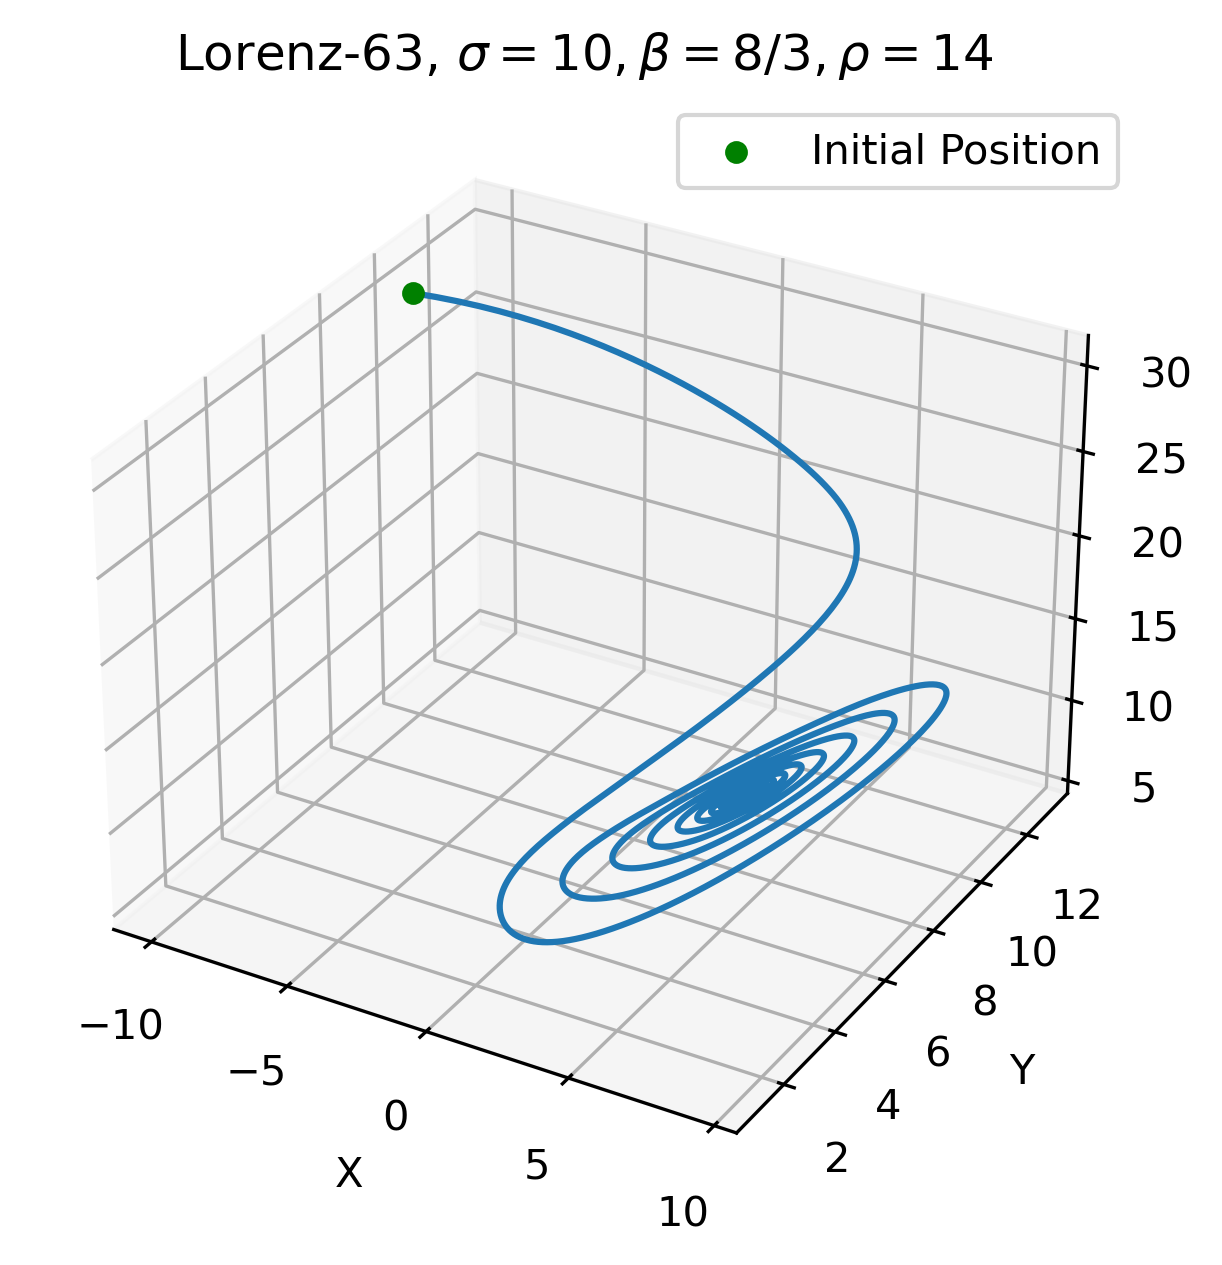
\includegraphics[scale=0.8]{graphics/Lorenz63_14.png}
    \caption{\textit{The evolution of the Lorenz-63 Model when $\sigma=10, \beta=8/3, \rho=14$ where the initial position is $\textbf{X} = (-10,10,30)^T$.}}
    \label{fig:lor63r14}
\end{figure}
\begin{figure}
    \centering
    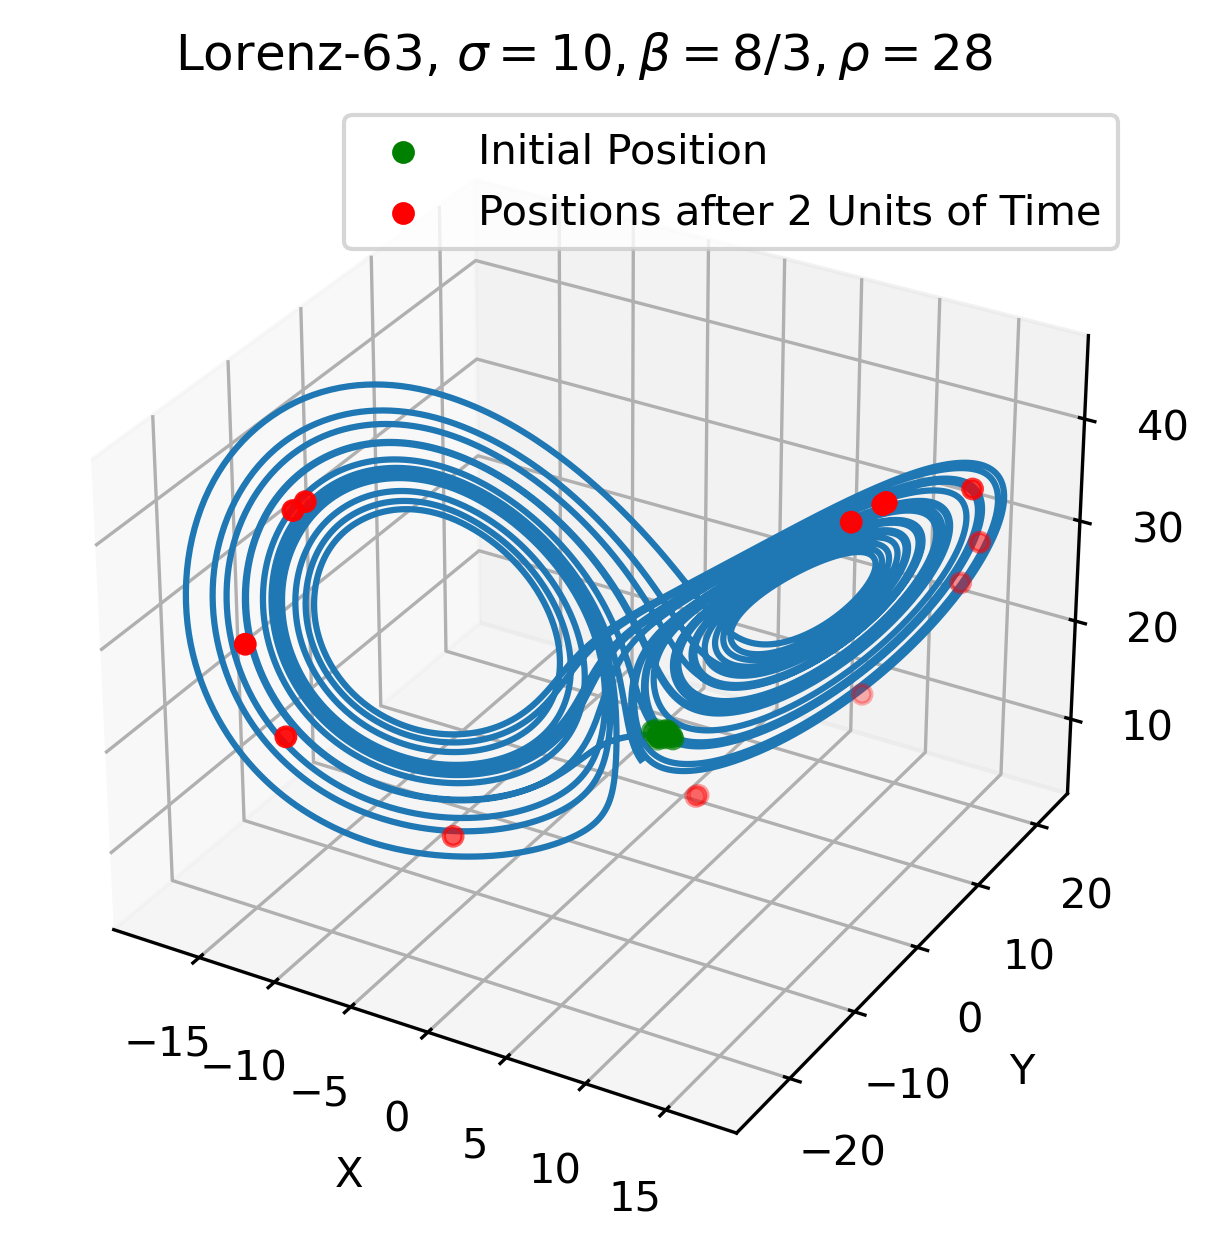
\includegraphics[scale=0.8]{graphics/Lorenz63_28.png}
    \caption{\textit{The evolution of the Lorenz-63 Model when $\sigma=10, \beta=8/3, \rho=28$ where the initial position is $\textbf{X} = (5,-5,20)^T$. An extra of 15 particles (overlapping green dots) are generated nearby and their positions after integration over 2 units of time are shown as red dots.}}
    \label{fig:lor63r28}
\end{figure}

\section{Python Programming}

In this section, we will show the necessary codes to produce Figures \ref{fig:lor63r14} and \ref{fig:lor63r28}. First, we need to use the \verb|solve_ivp| function from \verb|scipy.integrate| to integrate the dynamical system. We will define the equations of the Lorenz-63 Model as a function of $t$ and $\textbf{X}$ (which is denoted by the variable \verb|y| in the argument).
\begin{lstlisting}
import matplotlib.pyplot as plt
import numpy as np
from scipy.integrate import solve_ivp

def Lorenz63(t, y, sigma=10, beta=8/3, rho=14):
    X, Y, Z = y[0], y[1], y[2]
    dXdt = -sigma*X + sigma*Y
    dYdt = -X*Z + rho*X - Y
    dZdt = X*Y - beta*Z
    return([dXdt, dYdt, dZdt])
\end{lstlisting}
Then we will set the period of integration and the initial position of the particle.
\begin{lstlisting}
t_span = [0,25]
Y_0 = [-10,10,30]
\end{lstlisting}
Finally, we simply provide the defined \verb|Lorenz63| function for \verb|solve_ivp| to integrate.
\begin{lstlisting}
sol14 = solve_ivp(Lorenz63, t_span, Y_0, t_eval=np.linspace(t_span[0], t_span[1], 10000))
\end{lstlisting}
where \verb|t_eval| controls the frequency of sampling ($10000$ evenly spaced time steps here). To plot the results, we need to use the 3D projection and extract \verb|sol.y|:
\begin{lstlisting}
fig14 = plt.figure()
ax14 = plt.subplot(projection='3d')
ax14.set_title("Lorenz-63, " r"$\sigma=10, \beta=8/3, \rho=14$")
ax14.set_xlabel("X")
ax14.set_ylabel("Y")
ax14.set_zlabel("Z")
ax14.scatter(*Y_0, c="g", label="Initial Position")
ax14.plot(*sol14.y)
ax14.legend()
fig14.savefig("Lorenz63_14", dpi=300, bbox_inches="tight")
\end{lstlisting}
To run this with different parameters, we can give \verb|args| in \verb|solve_ivp|. Now we set $\rho = 28$ to enable chaotic behavior. The asterisk \verb|*| effectively expands the arrays into the three-directional components.
\begin{lstlisting}
Y_0 = [5,-5,20]
sol28 = solve_ivp(Lorenz63, t_span, Y_0, t_eval=np.linspace(t_span[0], t_span[1], 10000), args=(10,8/3,28))

# Other plotting commands are the same and hence omitted.
ax28.scatter(*Y_0, c="g", label="Initial Position")
ax28.plot(*sol28.y)
\end{lstlisting}
We will add some perturbations to the initial position of the particle via Gaussian noises. 15 new particles are generated in this way.
\begin{lstlisting}
n = 15
noises = np.random.multivariate_normal([0,0,0], np.diag([0.1]*3), n)
Ys_perturb = noises + Y_0    
\end{lstlisting}
We repeat the integration procedure for all particles. Their positions after 2 units of time are then plotted as well.
\begin{lstlisting}
Ys_t2 = np.full(Ys_perturb.shape, np.nan)
for ii in np.arange(n):
    sol_p = solve_ivp(Lorenz63, [0,2], Ys_perturb[ii,:], args=(10,8/3,28))
    Ys_t2[ii,:] = sol_p.y[:,-1]
    
# Other plotting commands are the same and hence omitted.
#ax28.scatter(*Ys_perturb.T, c="g")
ax28.scatter(*Ys_t2.T, c="r", label="Positions after 2 Units of Time")
fig28.savefig("Lorenz63_28", dpi=300, bbox_inches="tight")
\end{lstlisting}

\section{Exercises}

\begin{Exercise}
Determine the type of equilibrium point at the origin for the two-dimensional linear dynamical system $\textbf{y}' = A\textbf{y}$ where $A =$
\begin{enumerate}[label=(\alph*)]
    \item $\left[\begin{array}{@{\,}wc{12pt}wc{12pt}@{\,}}
    -1&-1\\ 
    0&-2
    \end{array}\right]$;
    \item $\left[\begin{array}{@{\,}wc{12pt}wc{12pt}@{\,}}
    0&-1\\ 
    2&2
    \end{array}\right]$;
    \item $\left[\begin{array}{@{\,}wc{12pt}wc{12pt}@{\,}}
    3&-2\\ 
    1&0
    \end{array}\right]$;
    \item $\left[\begin{array}{@{\,}wc{12pt}wc{12pt}@{\,}}
    1&-1\\ 
    -2&2
    \end{array}\right]$
\end{enumerate}
and find their general solution.
\end{Exercise}
\begin{Answer}
\begin{enumerate}[label=(\alph*)]
    \item Trace $= -3 < 0$, Determinant $= 2 > 0$, Discriminant $= (-3)^2 - 4(2) = 1 > 0$: Stable Node. The general solution is $\textbf{y} = c_1(1,0)^Te^{-t} + c_2(1,1)^Te^{-2t}$;
    \item Trace $= 2 > 0$, Determinant $= 2 > 0$, Discriminant $= 2^2 - 4(2) = -4 < 0$: Unstable Spiral. The general solution is $\textbf{y} = (c_1,c_2)^Te^t\cos(t) + (-c_1-c_2,2c_1+c_2)^Te^t\sin(t)$;
    \item Trace $= 3 > 0$, Determinant $= 2 > 0$, Discriminant $= 3^2 - 4(2) = 1 > 0$: Unstable Node. The general solution is $\textbf{y} = c_1(2,1)^Te^{2t} + c_2(1,1)^Te^{t}$;
    \item Trace $= 3 > 0$, Determinant $= 0$, Discriminant $= 3^2 - 4(0) = 9 > 0$: Degenerate case. The generals solution is $\textbf{y} = c_1(-1,2)^Te^{3t} + c_2(1,1)^T$.
\end{enumerate}
\end{Answer}

\begin{Exercise}
Describe the equilibrium point for the three-dimensional linear dynamical system $\textbf{y}' = A\textbf{y} + \textbf{G}$ where
\begin{align*}
A &= 
\begin{bmatrix}
-1&3&-1\\ 
1&1&-3\\ 
-2&2&-2
\end{bmatrix}
& & G=
\begin{bmatrix}
1 \\
-3 \\
2
\end{bmatrix}
\end{align*}
\end{Exercise}
\begin{Answer}
The equilibrium point is found by solving $A\tilde{\textbf{y}} = -G$ which gives $\tilde{\textbf{y}} = (\frac{3}{2}, 0, -\frac{1}{2})^T$. The eigenvalues of $A$ are $\lambda = 2, -2\pm 2i$ so it is an inward spiral on a cross-section that extends outwards along a cut-through axis.
\end{Answer}

\begin{Exercise}
Find all equilibrium points for the following two-dimensional non-linear dynamical system
\begin{empheq}[left={\empheqlbrace}]{alignat=1}
\frac{dx}{dt} &= x^2 - 2y^2 + xy \nonumber \\ 
\frac{dy}{dt} &= x^2 + y^2 - 1 \nonumber
\end{empheq}
and discuss their stability.
\end{Exercise}
\begin{Answer}
There are four equilibrium points: $\smash{(-\frac{1}{\sqrt{2}}, -\frac{1}{\sqrt{2}})^T}$, $\smash{(\frac{1}{\sqrt{2}}, \frac{1}{\sqrt{2}})^T}$, $\smash{(-\frac{2}{\sqrt{5}}, \frac{1}{\sqrt{5}})^T}$, and $\smash{(\frac{2}{\sqrt{5}}, -\frac{1}{\sqrt{5}})^T}$. The Jacobian matrix can be found as
\begin{align*}
\begin{bmatrix}
\dfrac{\partial F_1}{\partial x} & \dfrac{\partial F_1}{\partial y} \\[10pt]
\dfrac{\partial F_2}{\partial x} & \dfrac{\partial F_2}{\partial y}
\end{bmatrix} 
&= 
\begin{bmatrix}
\dfrac{\partial (x^2 - 2y^2 + xy)}{\partial x} & \dfrac{\partial (x^2 - 2y^2 + xy)}{\partial y} \\[10pt]
\dfrac{\partial (x^2 + y^2 - 1)}{\partial x} & \dfrac{\partial (x^2 + y^2 - 1)}{\partial y}
\end{bmatrix} \\
&= 
\begin{bmatrix}
2x + y & -4y + x \\
2x & 2y
\end{bmatrix}
\end{align*}
Take the first equilibrium point $\smash{(-\frac{1}{\sqrt{2}}, -\frac{1}{\sqrt{2}})^T}$ as an example, the values of the Jacobian matrix will be
\begin{align*}
\begin{bmatrix}
2(-\frac{1}{\sqrt{2}}) + (-\frac{1}{\sqrt{2}}) & -4(-\frac{1}{\sqrt{2}}) + (-\frac{1}{\sqrt{2}}) \\
2(-\frac{1}{\sqrt{2}}) & 2(-\frac{1}{\sqrt{2}})
\end{bmatrix} 
=
\begin{bmatrix}
-\frac{3}{\sqrt{2}} & \frac{3}{\sqrt{2}} \\
-\sqrt{2} & -\sqrt{2}
\end{bmatrix} 
\end{align*}
Its trace is $\smash{-\frac{5}{\sqrt{2}}} < 0$, the determinant is $6 > 0$ and the discriminant is $\smash{(-\frac{5}{\sqrt{2}})^2} - 4(6) = -\frac{23}{2} < 0$. Hence it is a stable spiral. Similarly, we can deduce that $\smash{(\frac{1}{\sqrt{2}}, \frac{1}{\sqrt{2}})^T}$ is an unstable spiral, while $\smash{(-\frac{2}{\sqrt{5}}, \frac{1}{\sqrt{5}})^T}$ and $\smash{(\frac{2}{\sqrt{5}}, -\frac{1}{\sqrt{5}})^T}$ are saddle points.
\end{Answer}

\begin{Exercise}
Examine the chaotic behavior of the \textit{Rössler attractor}:
\begin{subequations}
\begin{empheq}[left={\empheqlbrace}]{alignat=1}
\frac{dx}{dt} &= -y-z \\ 
\frac{dy}{dt} &= x+ay \\
\frac{dz}{dt} &= b+z(x-c)
\end{empheq}
\end{subequations}
with three parameters $a=0.2, b=0.2, c=5.7$ and plot it.
\end{Exercise}